%
%
\chapter{Mecânica Clássica}

\begin{enumerate}[start=1,label={\bfseries Q\arabic*.}]


\item Considere os arranjos de dois blocos de massas $m_{1}$ e $m_{2}$ ($m_{1} < m_{2}$) ilustrados nas figuras abaixo. Os coeficientes de atrito cinético entre cada bloco e o chão são $\mu_{1}$ e $\mu_{2}$, respectivamente. A aceleração da gravidade é $g$. Na Figura 1, uma força horizontal $\vec{F} = F(x)\hat{x}$ atua no bloco $m_{1}$ e o conjunto se move sem movimento relativo entre os blocos.


\begin{figure}[!ht]
	\centering
	\begin{minipage}{0.5\textwidth}
		\centering
		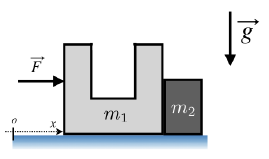
\includegraphics[width=0.7\textwidth]{classica-img/bloco1a.png} 
		\caption{Arranjo 1}
		\label{fig:bloco1apng}
	\end{minipage}\hfill
	\begin{minipage}{0.5\textwidth}
		\centering
		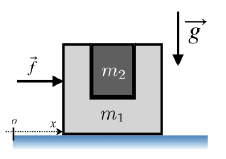
\includegraphics[width=0.7\textwidth]{classica-img/bloco2a.png}
		\caption{Arranjo 2}
		\label{fig:bloco2apng}
	\end{minipage}
\end{figure}



a) Indique esquematicamente todas as forças atuando em cada bloco da Figura 1.

\resposta

As figuras a baixo mostram as forças atuando em cada bloco.

\begin{figure}[H]
\centering
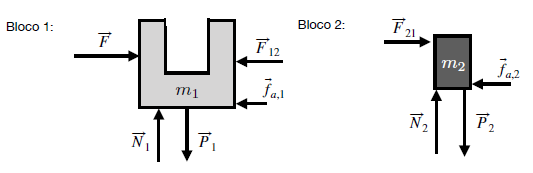
\includegraphics[scale=0.7]{classica-img/bloco1.png}
\end{figure}

As forças esquematizadas são as seguintes:

\begin{itemize}
\item[$\vec{F}_{ij}$]: Forças de contato entre os blocos (par de ação e reação: $\vec{F}_{ij}$ + $\vec{F}_{ji} = 0$).
\item[$\vec{f}_{a,i}$]: Força de atrito no $i$-ésimo bloco devido ao chão ($|\vec{f}_{a,i}| = \mu_{i} |\vec{N}_{i}|$).
\item[$\vec{N}_{i}$]: Força de reação normal no $i$-ésimo bloco devido ao chão.
\item[$\vec{P}_{i}$]: Força peso no $i$-ésimo bloco ($\vec{P}_{i} = m_{i}\vec{g}$).
\end{itemize}



b) Encontre a aceleração do bloco $m_{1}$ no caso da Figura \ref{bloco1png}. Dê sua resposta final em termos de $m_{1}$, $m_{2}$, $\mu_{1}$, $\mu_{2}$, $g$ e $F(x)$.

\resposta

Aplicando a segunda lei de Newton a cada um dos blocos e usando que os blocos movem-se com a mesma aceleração horizontal $a_{x}$

\begin{itemize}
\item na direção de x: $F(x) - F_{1,2} - f_{a,1} = m_{1}a_{x}$ \quad e \quad $F_{2,1} - f_{a,2} = m_{2}a_{x}$,

\item na direção y: $N_{1} = P_{1} \Rightarrow N_{1} = m_{1}g $ \quad e \quad $N_{2} = P_{2} \Rightarrow N_{2} = m_{2}g $.

$$
\left\{
\begin{array}{ccc}
	F(x) - F_{1,2} - f_{a,1} & = & m_{1} a_{x} \\
	       F_{2,1} - f_{a,2} & = & m_{2} a_{x}
\end{array}
\right.
$$

Do sistema acima as forças de contato se anulam. Isolando $a_{x}$

$$
\Rightarrow a_{x}  = \frac{F(x) - g(\mu_{1}m_{1} + \mu_{2} m_{2})}{m_{1} + m_{2}}
$$
\end{itemize}

c) Encontre a variação da energia cinética do arranjo da Figura 1 se a posição do bloco de massa $m_{1}$ variar de $x_{1}$ até $x_{2}$ ($x_{2} > x_{1}$) e se $F(x) = \alpha x$, onde $\alpha$ é uma constante positiva.

\resposta

Do teorema trabalho-energia cinética, sabe-se que a variação total da energia cinética é igual ao trabalho da força resultante $\vec{F}_{R}$ sobre o sistema. Esta é dada por

$$
\vec{F}_{R} = [F(x) - g(\mu_{1}m_{1} + \mu_{2}m_{2})] \hat{x}
$$

$$
\vec{F}_{R} = [\alpha x - g(\mu_{1}m_{1} + \mu_{2}m_{2})] \hat{x}.
$$

Segue que a variação da energia cinética $\Delta K$ entre as posições $x_{1}$ e $x_{2}$ é

$$
\Delta K = \int_{x_{2}}^{x_{1}} \vec{F}_{R} \cdot d\vec{l} = \frac{\alpha}{2} (x_{2}^{2} - x_{1}^{2}) - g(\mu_{1}m_{1} + \mu_{2}m_{2})(x_{2} - x_{1})
$$

d) Considere agora que ambos os conjuntos das Figuras 1 e 2 se movam instantaneamente com a mesma velocidade $v$ e que a potência dissipada por atrito no arranjo da Figura 2 seja o dobro da do arranjo da Figura 1. Encontre a razão $\mu_{2}/\mu_{1}$.

\resposta

A potência total instantânea dissipada pelo atrito é $P = \vec{f}_{a,tot} \cdot \vec{v} = - f_{a,tot} v$, onde $\vec{f}_{a,tot}$ é a força de atrito total atuando no sistema. Impondo-se a condição do enunciado $P_{fig,2} = 2P_{fig,1}$ e usando

$$
 \vec{f}_{a,tot,fig,1} = \vec{f}_{a,1} + \vec{f}_{a,2} = g(\mu_{1}m_{1} + \mu_{2}m_{2})\hat{x} \Rightarrow \mbox{Arranjo da Fig 1}
$$

$$
 \vec{f}_{a,tot,fig,2} = g\mu_{1}(m_{1} + m_{2}) \hat{x} \Rightarrow \mbox{Arranjo da Fig 2}
$$

Como $P_{fig,2} = 2P_{fig,1}$ obtém-se

$$
\mu_{1}(m_{1} + m_{2}) = 2(\mu_{1}m_{1} + \mu_{2}m_{2}) \Rightarrow \frac{\mu_{2}}{\mu_{1}} = \frac{m_{2} - m_{1}}{2m_{2}}
$$



\item Um pêndulo de comprimento l e massa $m$ está preso a um bloco de massa $M$. O bloco é livre para se mover sem atrito ao longo de um trilho horizontal, conforme indicado na figura. Considere a posição $y = 0$ ($\theta = \pi/2$) como o zero de energia potencial gravitacional. A aceleração da gravidade é $g$.

\begin{figure}[H]
\centering
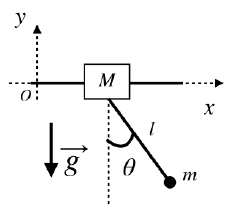
\includegraphics[scale=0.5]{classica-img/pendulo.png}
\end{figure}


a) Escreva a lagrangiana do sistema em termos das coordenadas generalizadas $x$ (posição do bloco) e $\theta$ (ângulo que o pêndulo faz com a vertical) mostradas na figura. Encontre as equações de movimento.

\resposta

No sistema de referência do enunciado, as posições do bloco de massa $M$ e da massa do pêndulo $m$ são dadas, respectivamente, por $\vec{r}_{M} = x(t)\hat{i}$ e $\vec{r}_{m} = [x(t) + l sen\theta(t)]\hat{i} - l cos\theta(t)\hat{j}$. Deste modo,

$$
v_{m}^{2} = \left| \frac{d\vec{r}_{m}}{dt} \right|^{2} = \left( \dot{x} + l\dot{\theta} cos \theta  \right)^{2} + \left( l\dot{\theta} sen \theta \right)^{2} = \dot{x}^{2} + l^{2} \dot{\theta}^{2} + 2 l\dot{\theta}\dot{x}cos \theta
$$

Portanto, adotando a posição $y = 0$ ($\theta = \pi/2$) como o zero de energia potencial gravitacional, a lagrangiana do sistema é dada por

$$
L = \frac{1}{2} M \dot{x}^{2} + \frac{1}{2} m \left( \dot{x}^{2} + l^{2} \dot{\theta}^{2} 2 l\dot{\theta}\dot{x}cos \theta   \right) + mlg \ cos \theta.
$$

Das equações de Euler-Lagrange, as equações de movimento são

\begin{eqnarray}
(m + M) \ddot{x} + (ml \cos \theta) \ddot{\theta} - (ml \ sen \theta) \dot{\theta}^{2} &=& 0 \\
l \ddot{\theta} + cos \theta \ddot{x} + g sen \theta &=& 0
\end{eqnarray}


b) Além da energia mecânica total, existe alguma outra constante de movimento na dinâmica do sistema?          Qual? Justifique.

\resposta

Sim, a componente $x$ do momentum linear total do sistema $P_{x}$ se conserva. Isto decorre do fato de que a força total no sistema só tem componente na direção $y$. De fato,

\begin{eqnarray*}
P_{x} &=& (\vec{p}_{M} + \vec{p}_{m})\cdot \hat{i} = M\dot{x} + m (\dot{x} + l \dot{\theta} cos \theta) \\
\Rightarrow \frac{dP_{x}}{dt} &=& (m+M)\ddot{x} + (mlcos\theta)\ddot{\theta} - (mlsen\theta)\dot{\theta}^{2} = 0,
\end{eqnarray*}

onde usamos a Eq. (1) no último passo. Alternativamente, percebe-se que a coordenada $x$ é ignorável, ou seja, a lagrangiana não depende de $x$. Portanto, o momento canonicamente conjugado a $x$, que é o lado esquerdo da Eq. (1), é conservado.


c) Considerando o regime de pequenas oscilações ($\theta << 1$), encontre o modo normal de oscilação do sistema e a sua frequência.

\resposta

Com $\theta << 1$ ($sen \theta \approx \theta$ e $cos \theta \approx 1$), as equações de movimento podem ser linearizadas

\begin{eqnarray}
(m+M)\ddot{x} + ml\ddot{\theta} &\approx & 0, \\
\ddot{x} + l\ddot{\theta} + g \theta &=& 0.
\end{eqnarray}

Isolando a equação para $\theta$, obtém-se

$$
\ddot{\theta} + \left( \frac{m+M}{M}  \right) \frac{g}{l} \theta = 0,
$$


cuja solução geral é $\theta (t) = A cos (\omega t + \varphi)$, onde $\omega = \sqrt{\frac{m+M}{M} \frac{g}{l}}$ e $A$ e $\varphi$ são constantes determinadas pelas condições iniciais. Integrando duas vezes a Eq. (3) em relação ao tempo obtém-se

$$
x(t) = -\frac{ml}{m+M} \theta l + Bt + C,
$$

Nesse modo, o bloco $M$ e a massa $m$ oscilam com a mesma frequência $\omega$ mas em sentidos opostos (além de um movimento do centro de massa do sistema com velocidade constante na direção $x$).



d) Além do caso trivial no qual o sistema está parado ($\dot{x} = 0$, $\dot{\theta} = 0$), existe algum outro movimento possível em que o pêndulo não oscile? Qual? Justifique.

\resposta

Sim. Fazendo $A = 0$ na solução do item (c), obtém-se $\theta(t) = 0$ e $x(t) = Bt + C$, isto é, o sistema se move com um todo com velocidade constante $B$, com o pêndulo sempre na vertical $\theta = 0$. Este é o outro modo normal do problema, cuja frequência de oscilação é nula. Deve-se notar que essa é uma solução exata das Eqs. de movimento (1) e (2).






\item A figura abaixo mostra esquematicamente um sistema formado pelo bloco 1, de massa $m_{1} = 2m$, conectado a uma mola de constante elástica $k$ e massa desprezível, e pelo bloco 2, de massa $m_{2} = m$. No instante inicial o bloco 1 está em repouso, a mola encontra-se relaxada, e o bloco 2 movimenta-se em direção ao bloco 1 com velocidade $\vec{v}_{2,1} = - v_{0} \hat{x}$, sendo $v_{0} > 0$. Os dois blocos colidem elasticamente elasticamente e o bloco 1 passa a oscilar após a colisão. Há atrito entre os blocos e a superfície \textbf{apenas no trecho inclinado AB} e o módulo da aceleração da gravidade vale $g$.

\begin{figure}[H]
\centering
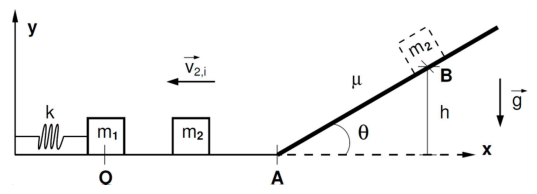
\includegraphics[scale=0.5]{classica-img/inclinado.png}
\end{figure}


a) Determine, em termos de $v_{0}$, os \textbf{vetores} velocidade dos blocos 1 e 2 imediatamente após a colisão ($\vec{v}_{1,f}$ e $\vec{v}_{2,f}$). Assuma que a mola não afeta o processo de colisão.

\resposta


b) Determine a amplitude $x_{m}$ do movimento oscilatório do bloco 1 após a colisão em termos de $m$, $k$ e $v_{0}$.

\resposta

c) Após a colisão, o bloco 2 movimenta-se em direção ao plano inclinado e atinge o repouso permanente no ponto B. Determine o coeficiente de atrito cinético $\mu$ entre o bloco 2 e o trecho inclinado AB em termos de $g$, $v_{0}$, da altura $h$ e do ângulo $\theta$

\resposta

d) Indique esquematicamente todas as forças que atuam no bloco 2 quando ele se encontra em repouso no ponto B.

\resposta



\item Uma barra longa e de massa desprezível movimenta-se no plano xy girando em torno do eixo z com velocidade angular constante $\omega$, como mostrado na figura abaixo. Uma partícula de massa $m$ pode deslizar sem atrito ao longo da barra, e sofre a ação de uma força externa $\vec{F} = m\gamma \hat{x}$, sendo $\gamma$ uma constante positiva.

\begin{figure}[H]
\centering
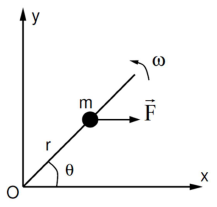
\includegraphics[scale=0.8]{classica-img/barra.png}
\end{figure}



a) Determine a energia potencial $V(\vec{r})$ associada à força $\vec{F}$. Considere a origem O como sendo o ponto de energia potencial nula.

\resposta

b) Determine a equação do vínculo em termos das coordenadas polares, $r$ e $\theta$, e do tempo $t$. Qual é a origem física da correspondente força de vínculo?

\resposta

c) Escreva a Lagrangiana da partícula em termo da coordenada $r$, da sua derivada temporal $\dot{r}$, e do tempo $t$. Em seguida, determine a correspondente equação de movimento.

\resposta

d) Considere o caso em que $\gamma = 0$ e determine a solução geral da equação de movimento calculada no item (c). Em seguida, determine a componente radial $r(t)$ da posição da partícula em funão do tempo. Incialmente, $r(t=0)=a$ e $\dot{r}(t=0)=0$.

\resposta




\item Um carro se move numa pista circular inclinada de um ângulo $\theta$ em relação à horizontal. A figura abaixo mostra o plano transversal ao movimento do carro. O módulo da aceleração da gravidade é $g$.
\begin{figure}[H]
\centering
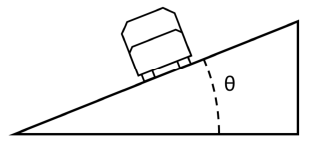
\includegraphics[scale=0.8]{classica-img/inclina}
\end{figure}



a) Indique esquematicamente todas as forças que atuam no carro, se o atrito for desprezível.

\resposta As forças que atuam no carro são a normal $\mathbb{N}$ e o peso $\mathbb{P}$, como mostrado na figura abaixo.
\begin{figure}[H]
\centering
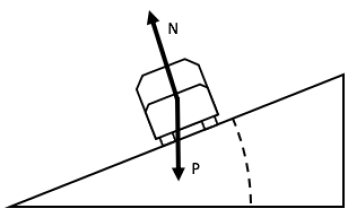
\includegraphics[scale=0.8]{classica-img/inclina1}
\end{figure}


b) Ainda desprezando o atrito, encontre o módulo da velocidade com a qual o carro se move, se ele descreve um círculo de raio $R$.

\resposta Tomando um sistema de referência fixo na pista e com origem na posição instantânea do carro com o eixo $z$ na direção vertical, teremos equilíbrio na direção $z$
$$
N \cos \theta = m g
$$
onde $m$ é a massa do carro. No plano $xy$ o carro realiza um movimento circular uniforme com velocidade $v$ cuja resultante centrípeta é
$$
N \sin \theta = \frac{mv^{2}}{R}.
$$
Eliminando $\mathbf{N}$ das Eqs. (1) e (2),
$$
v = \sqrt{gR\tan \theta}
$$

c) A partir deste item, considere que haja atrito entre os pneus do carro e a pista e que o coeficiente de atrito estático seja $\mu$. Se o carro se move com a velocidade máxima possível sem derrapar, indique esquematicamente todas as forças que atuam no carro.

\resposta Se $\mathbf{F}_{at}$ é a força de atrito, o diagrama de forças agora é
\begin{figure}[H]
\centering
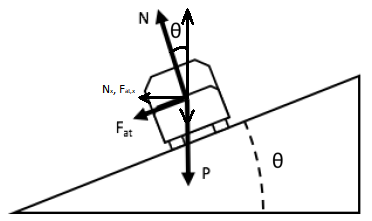
\includegraphics[scale=0.8]{classica-img/inclina2}
\end{figure}



d) Qual é o módulo da velocidade máxima com a qual o carro é capaz de fazer a curva de raio $R$ sem derrapar?

\resposta Usando o mesmo sistema de referência do item (b), ainda há equilíbrio na direção $z$
$$
N \cos \theta=m g+F_{a t} \sin \theta=m g+\mu N \sin \theta
$$
onde já usamos que, no limiar da derrapagem, a força de atrito estático $F_{at}$ atinge seu valor máximo, $\mu N$. A resultante centrípeta no plano $xy$ agora é
$$
N \sin \theta+F_{a t} \cos \theta=N \sin \theta+\mu N \cos \theta=\frac{m v_{\max }^{2}}{R}
$$
onde $v_{max}$ é a velocidade máxima sem derrapar. Eliminando novamente $N$ das Eqs. (3) e (4),
$$
v_{\max }=\sqrt{g R\left(\frac{\tan \theta+\mu}{1-\mu \tan \theta}\right)}.
$$

e) Suponha agora que $sin \ \theta > \mu cos \theta$ e que o carro se mova bem mais lentamente. Indique esquematicamente todas as forças que atuam no carro nesse caso. Determine a velocidade mínima com a qual o carro consegue descrever o círculo de raio $R$ sem derrapar.

\resposta Nesse caso, o sentido da força de atrito se inverte
\begin{figure}[H]
\centering
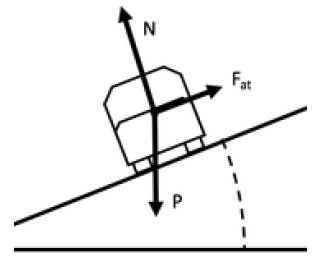
\includegraphics[scale=0.8]{classica-img/inclina3}
\end{figure}
O desenvolvimento do item (d) se repete bastando inverter o sinal de $\mu \rightarrow - \mu$ e a velocidade máxima sem derrapar $v_{min}$ é
$$
v_{\min }=\sqrt{g R\left(\frac{\tan \theta-\mu}{1+\mu \tan \theta}\right)}
$$
Note que o enunciado diz que $\tan \theta > \mu$, o que garante que o resultado obtido é um número real. Do contrário, o carro consegue ficar em repouso na pista, pois o ângulo é menor que o ângulo crítico $\theta_{c} = \arctan(\mu)$ e $v_{min} = 0$.







\item Considere um pêndulo constituído por um pequeno corpo de massa $m$ suspenso por uma mola de massa desprezível e constante elástica $k$. O comprimento de equilíbrio da mola (sem nenhuma massa pendurada) é $l$. Considere que o movimento do pêndulo esteja sempre contido num plano vertical fixo. Utilize coordenadas generalizadas tais que o comprimento da mola seja $l + r(t)$ e o ângulo desta com a vertical seja $\theta(t)$.


a) Escreva a energia cinética do sistema em termos de $r$, $\theta$ e suas derivadas temporais.

\resposta Suponha um sistema de referência tal que o plano $xy$ contenha o movimento do pêndulo, que sua origem esteja no ponto de sustentação do pêndulo e que o eixo $y$ seja vertical para cima. As relações entre as coordenadas cartesianas do corpo e $r$ e $\theta$ são
$$
x=(l+r) \sin \theta \ \ \ \mbox{e} \ \ \ y=-(l+r) \cos \theta
$$
A energia cinética assume a forma
$$
T=\frac{1}{2} m v^{2}=\frac{1}{2} m\left(\dot{x}^{2}+\dot{y}^{2}\right)=\frac{1}{2} m\left(\dot{r}^{2}+(r+l)^{2} \dot{\theta}^{2}\right)
$$

b) Escreva a energia potencial do sistema em termos de $r$, $\theta$ e suas derivadas temporais.

\resposta A energia potencial do sistema está associada à mola, $U_{mola}$, e ao campo gravitacional $g = - g \hat{y}$, $U_{g}$. Como o comprimento de equilíbrio da mola é igual a $l$
$$
U_{mola} = \frac{1}{2} kr^{2} \  \  \  \mbox{e} \  \  \ U_{g} = mgy = - mg(r+l)\cos \theta.
$$
Dessa forma,
$$
U = U_{mola} + U_{g} = \frac{1}{2} kr^{2} - mg(r+l)\cos \theta.
$$


c) Escreva a lagrangiana do sistema.

\resposta  Utilizando os resultados dos itens (a) e (b) a lagrangiana da partícula é dada por
$$
L = T - U = \frac{1}{2}m \left( \dot{r}^{2} + (r+l)^{2} \dot{\theta}^{2} \right) - \frac{1}{2} kr^{2} + mg(r+l)\cos \theta.
$$



d) Escreva as equações de Euler-Lagrange para $r$ e $\theta$.

\resposta Primeiramente,

$$
\begin{aligned}
\frac{\partial L}{\partial r} &=m(r+l) \dot{\theta}^{2}-k r+m g \cos \theta \\
\frac{\partial L}{\partial \dot{r}} &=m \dot{r} \\
\frac{\partial L}{\partial \theta} &=-m g(r+l) \sin \theta \\
\frac{\partial L}{\partial \dot{\theta}} &=m(r+l)^{2} \dot{\theta}
\end{aligned}
$$
As Eqs. de Euler-Lagrange são
$$
\begin{aligned}
&\frac{\partial L}{\partial r}-\frac{d}{d t}\left(\frac{\partial L}{\partial \dot{r}}\right)=0 \rightarrow \ddot{r}-(r+l) \dot{\theta}^{2}-g \cos \theta+\frac{k}{m} r=0\\
&\frac{\partial L}{\partial \theta}-\frac{d}{d t}\left(\frac{\partial L}{\partial \dot{\theta}}\right)=0 \quad \rightarrow \quad(r+l) \ddot{\theta}+2 \dot{r} \dot{\theta}+g \sin \theta=0
\end{aligned}
$$

e) Considere agora o movimento puramente vertical do pêndulo, ou seja, $\theta(t) = 0$ para todo $t$. Encontre a solução geral (em termos de duas constantes arbitrárias) da equação de Euler-Lagrange para $r$.

\resposta A equação de movimento (5) para $\theta = \dot{\theta} = 0$ assume a forma
$$
\ddot{r} + \frac{k}{m} r = g.
$$
A solução geral da Eq. (7) é dada por
$$
r(t) = r_{H}(t) + r_{P}(t)
$$
onde $r_{H}(t)$ é a solução geral da equação homogênea (ou seja, fazendo $g = 0$ na Eq. (7)) e $r_{P}(t)$ é uma solução particular qualquer da equação não homogênea. Como a equação homogênea é igual à equação de movimento do oscilador harmônico simples, temos que
$$
r_{H}(t) = A \cos \omega t + B \sin \omega t,
$$
onde $\omega = \sqrt{k/m}$ e $A$ e $B$ são constantes arbitrárias determinadas a partir das condições iniciais. Como o termo não homogêneo é constante, tentamos uma solução da forma
$$
r_{P}(t) = Ct^{2} + Dt + E.
$$
Substituindo na Eq. (7), verifica-se que as constantes $C = D = 0$ e $E = g/\omega^{2} = mg/k$. Assim,
$$
r_{P}(t) = \frac{g}{\omega^{2}} = \frac{mg}{k}.
$$
Por fim, a solução geral da Eq. (7) é dada por
$$
r(t) = A \cos \omega t + B \sin \omega t + \frac{mg}{k}.
$$








\item Uma partícula de massa $m$  movimenta-se num plano vertical (plano $xz$, sendo $x$ a direção horizontal e $z$ a direção vertical) sob a ação da força gravitacional $\mathbf{F}_{g} = m \mathbf{g} = - m g \hat{\mathbf{z}}$, onde $g$ é a aceleração da gravidade. No instante inicial $t=0$, a partícula está na origem e sua velocidade é $\mathbf{v}_{0} = (v_{0} cos \theta) \hat{\mathbf{x}} + (v_{0} sen \theta) \hat{\mathbf{z}}$, onde $v_{0} > 0$ e $0 < \theta < \pi/4$.



a) Escreva as equações de movimento para as componentes $x$ e $z$ da posição da partícula.

\resposta

b) Determine as componentes $v_{x}(t)$ e $v_{z}(t)$ da velocidade da partícula como funções do tempo.

\resposta

c) Determine as componentes $x(t)$ e $z(t)$ da posição da partícula como funções do tempo.

\resposta

d) Determine o \textbf{vetor} momento angular $\mathbf{L}(t)$ da partícula em relação à origem como função do tempo.

\resposta

e) Determine o \textbf{vetor} torque $\mathbf{N}(t)$ em relação à origem associado à força gravitacional $\mathbf{F}_{g}$ (como função do tempo) e encontre a relação entre $\mathbf{L}(t)$ e $\mathbf{N}(t)$.

\resposta




\item Uma partícula de massa $m$ movimenta-se em duas dimensões (plano $xy$) sob a ação de duas forças conservativas cujos potenciais são

$$
U_{1}(y) = \lambda y \quad  \mbox{ e } \quad U_{2}(r) = \frac{1}{2} kr^{2},
$$

onde $\lambda$ e $k$ são constantes positivas e $r = \sqrt{x^{2} + y^{2}}$ é a distância da partícula à origem do sistema de coordenadas.


a) Determine o \textbf{vetor} força $\mathbf{F}_{2}$ associada ao potencial $U_{2}(r)$.

\resposta

b) Escreva a lagrangiana da partícula utilizando coordenadas polares no plano $r$ e $\theta$ e determine as equações de movimento correspondentes.

\resposta

c) Encontre a hamiltoniana do sistema. Lembre-se de que a hamiltoniana deve ser escrita dem termos das coordenadas $r$ e $\theta$ e dos seus momentos canonicamente conjugados.

\resposta

d) Encontre o \textbf{vetor} momento angular $\mathbf{L}$ em termos das coordenadas polares $r$ e $\theta$. Determine sob qual condição o momento angular da partícula é conservado.

\resposta




\item Um disco fino homogêneo de raio $R$ e massa m move-se ao longo de uma superfície horizontal. O coeficiente de atrito cinético entre o disco e a superfície horizontal é $\mu$. No instante inicial (ver figura abaixo), a coordenada $x$ do centro do disco está em O, a velocidade do seu centro
$\mathbf{v}_{0} = v_{0}\hat{\mathbf{x}}$ e a velocidade angular de rotação (em torno do eixo que passa pelo centro de massa e é normal ao disco) é nula. \textbf{Apenas quando atinge o ponto A o disco passa a rolar sem deslizar}: enquanto a coordenada $x$ do seu centro percorre o trecho de O até A, a
força de atrito cinético age de forma a mudar tanto a velocidade do centro de massa quanto a velocidade angular de rotação. Considere que o plano do disco se mantém paralelo ao plano $xy$ e a aceleração da gravidade é $\mathbf{g} -g\hat{\mathbf{y}}$.

\begin{figure}
\centering
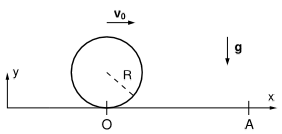
\includegraphics[scale=1]{classica-img/disco.png}
\end{figure}


a) Indique esquematicamente todas as forças que atuam sobre o disco no trecho OA.

\resposta

b) Determine os \textbf{módulos} das acelerações linear $a$ e angular $\alpha$ do disco em termos de $R$, $\mu$ e $g$ no trecho OA. O momento de inércia do disco em relação ao eixo que passa pelo seu centro e é normal ao plano do disco é $I = mR^{2}/2$.

\resposta

c) Determine os \textbf{módulos} das velocidades linear $v$ e angular $\omega$ do disco para o trecho OA como funções do tempo.

\resposta

d) Escreva a relação entre os \textbf{módulos} das velocidades linear $v$ e angular $\omega$ do disco quando ele passa a rolar sem deslizar (ponto A). Em seguida, determine o instante de tempo $t_{A}$ em que a coordenada $x$ do centro do disco atinge o ponto A. Expresse sua resposta em termos de $v_{0}$, $\mu$ e $g$.

\resposta







\item Considere uma partícula de massa $m$ que se movimenta na superfície interna de um cone cuja ponta é a origem do sistema de coordenadas e cujo eixo é o semi-eixo $z > 0$. A equação da superfície do cone em coordenadas cilíndricas ($\rho, \varphi e z$) é $z = \rho$. A partícula está sob a ação do campo gravitacional $\mathbf{g} = —g\hat{\mathbf{z}}$.


a) Escreva a lagrangiana da partícula em termos de $\rho, \varphi, \dot{\rho} e \dot{\rho}$

\resposta

b) Determine as equações de movimento da partícula.

\resposta

c) Calcule o $\mathbf{vetor}$ momento angular da partícula $\mathbf{L}$ em termos das coordenadas cilíndricas $\rho$, $\phi$ e $z$ e dos vetores unitários $\hat{\mathbf{\rho}}$, $\hat{\mathbf{\phi}}$ e $\hat{\mathbf{z}}$. Determine qual componente de $\mathbf{L}$ é conservada.

\resposta

d) A partir das equações de movimento derivadas no item (b), mostre que a partícula pode apresentar uma órbita circular de raio $\rho_{0}$. Determine a frequência angular dessa órbita em termos de $g$ e $\rho_{0}$ Determine a frequência angular dessa órbita em termos de $g$ e $\rho_{0}$.

\resposta





\item Um corpo de massa $m$ cai em linha reta a partir do repouso em um fluido. A aceleração da gravidade $\vec{g}$ pode considerada constante. O corpo é sujeito também a uma força de resistência proporcional à velocidade: $\vec{F}_{r} = -km\vec{v}$, onde $k$ é uma constante. A força de empuxo do fluido é desprezível.


a) Obtenha o módulo da velocidade do corpo como função do tempo.

\resposta Da componente da segunda lei de Newton na direção vertical (orientada para cima), a queda é descrita por
$$
F=m \frac{d v}{d t}=-m g-k m v \Rightarrow \frac{d v}{d t}=-(g+k v) \Rightarrow \int_{0}^{v} \frac{d v^{\prime}}{g+k v^{\prime}}=-\int_{0}^{t} d t^{\prime}
$$
onde usamos a condição inicial de que o corpo parte do repouso. Usando
$$
\int \frac{d x}{a x+b}=\frac{1}{a} \ln (a x+b)
$$
segue que
$$
\int_{0}^{v} \frac{d v^{\prime}}{g+k v^{\prime}}=-\int_{0}^{t} d t^{\prime} \Rightarrow \ln \left(\frac{g+k v}{g}\right)=-k t
$$
Invertendo a última relação
$$
v(t)=\frac{g}{k}\left(e^{-k t}-1\right)
$$
Como $v(t)<0$ (corpo em queda), o módulo da velocidade é
$$
|v(t)|=-\frac{g}{k}\left(e^{-k t}-1\right)=\frac{g}{k}\left(1-e^{-k t}\right)
$$

b) Qual é a velocidade terminal do corpo (módulo da velocidade no limite $t \rightarrow \infty$)?

\resposta A velocidade terminal $v_{\text {term}}$ é obtida tomando-se o limite $t \rightarrow \infty$ na Eq. (3)
$$
v_{\text {term}}=\lim _{t \rightarrow \infty} \frac{g}{k}\left(e^{-k t}-1\right)=-\frac{g}{k} \Rightarrow\left|v_{\text {term}}\right|=\frac{g}{k}
$$

c) Encontre $z(t)$, a posição do corpo como função do tempo (considere $z(0) = 0$).

\resposta A posição vertical do corpo é obtida integrando mais uma vez a Eq.
$$
v=\frac{d z}{d t}=\frac{g}{k}\left(e^{-k t}-1\right) \Rightarrow \frac{k}{g} \int_{0}^{z} d z^{\prime}=\int_{0}^{t}\left(e^{-k t^{\prime}}-1\right) d t^{\prime} \Rightarrow \frac{k z}{g}=-\frac{e^{-k t}}{k}+\frac{1}{k}-t
$$
donde
$$
z(t)=\frac{g}{k^{2}}\left(1-e^{-k t}\right)-\frac{g t}{k}
$$

d) Encontre $z(v)$, a posição do corpo como função do módulo da velocidade.

\resposta Das Eqs. (3) e (4)
$$
z=-\frac{v}{k}-\frac{g}{k} t
$$
Eliminando $t$ usando a Eq. $(2),$ encontramos a expressão procurada
$$
z(v)=\frac{g}{k^{2}} \ln \left(1+\frac{k v}{g}\right)-\frac{v}{k}
$$
Alternativamente, da Eq. ( 1 )
$$
a=\frac{d v}{d t}=-(g+k v)
$$
Mas
$$
\frac{d v}{d z}=\frac{d v}{d t} \frac{d t}{d z}=\frac{a}{v} \Rightarrow v d v=a d z=-(g+k v) d z
$$
Logo
$$
-\int_{0}^{v} \frac{v^{\prime}}{g+k v^{\prime}} d v^{\prime}=\left.\int_{0}^{z} d z^{\prime} \Rightarrow \frac{g \ln (g+k v)-k v}{k^{2}}\right|_{0} ^{v}=\left.z\right|_{0} ^{z}
$$
onde usamos o resultado $\int \frac{x}{a+b x} d x=\frac{b x-a \ln (a+b x)}{b^{2}} .$ Segue que
$$
z(v)=\frac{g}{k^{2}} \ln \left(1+\frac{k v}{g}\right)-\frac{v}{k}
$$




\item O pêndulo duplo plano consiste de duas partículas de massas $m_{1}$ e $m_{2}$ e duas hastes rígidas de massas desprezíveis e comprimentos $l_{1}$ e $l_{2}$, que oscilam, sob a ação da gravidade $\vec{g}$, em um mesmo plano vertical fixo, como representado na figura abaixo. Considerando $\vec{g}$ constante e adotando como coordenadas generalizadas os ângulos $\theta_{1}$ e $\theta_{2}$ da figura, obtenha:

\begin{figure}[H]
\centering
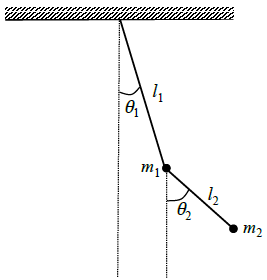
\includegraphics[scale=1]{classica-img/pendulo2.png}
\end{figure}


a) A energia cinética do sistema.

\resposta Seja um sistema cartesiano de coordenadas com $x$ na horizontal orientada para a direita e $y$ na vertical orientada para baixo e com a origem no ponto de sustentação do pêndulo superior. Sejam $\left(x_{1}, y_{1}\right) \mathrm{e}\left(x_{2}, y_{2}\right)$ as coordenadas cartesianas das partículas de massas $m_{1} \mathrm{e} m_{2}$ respectivamente. Então,
$$
x_{1}=l_{1} \sin \theta_{1}, \quad y_{1}=l_{1} \cos \theta_{1}, \quad x_{2}=l_{1} \sin \theta_{1}+l_{2} \sin \theta_{2}, \quad y_{2}=l_{1} \cos \theta_{1}+l_{2} \cos \theta_{2}
$$
donde
$$
\begin{aligned}
\dot{x}_{1} &=l_{1} \dot{\theta}_{1} \cos \theta_{1}, \quad \dot{x}_{2}=l_{1} \dot{\theta}_{1} \cos \theta_{1}+l_{2} \dot{\theta}_{2} \cos \theta_{2} \\
\dot{y}_{1} &=-l_{1} \dot{\theta}_{1} \sin \theta_{1}, \quad \dot{y}_{2}=-l_{1} \dot{\theta}_{1} \sin \theta_{1}-l_{2} \dot{\theta}_{2} \sin \theta_{2}
\end{aligned}
$$
A energia cinética da partícula $1 é$
$$
T_{1}=\frac{m_{1}}{2}\left(\dot{x}_{1}^{2}+\dot{y}_{1}^{2}\right)=\frac{m_{1}}{2}\left(l_{1}^{2} \dot{\theta}_{1}^{2} \cos ^{2} \theta_{1}+l_{1}^{2} \dot{\theta}_{1}^{2} \sin ^{2} \theta_{1}\right)=\frac{m_{1}}{2} l_{1}^{2} \dot{\theta}_{1}^{2}
$$
Para a partícula 2
$$
\begin{array}{l}
\dot{x}_{2}^{2}=l_{1}^{2} \dot{\theta}_{1}^{2} \cos ^{2} \theta_{1}+l_{2}^{2} \dot{\theta}_{2}^{2} \cos ^{2} \theta_{2}+2 l_{1} l_{2} \dot{\theta}_{1} \dot{\theta}_{2} \cos \theta_{1} \cos \theta_{2} \\
\dot{y}_{2}^{2}=l_{1}^{2} \dot{\theta}_{1}^{2} \sin ^{2} \theta_{1}+l_{2}^{2} \dot{\theta}_{2}^{2} \sin ^{2} \theta_{2}+2 l_{1} l_{2} \dot{\theta}_{1} \dot{\theta}_{2} \sin \theta_{1} \sin \theta_{2}
\end{array}
$$
donde
$$
T_{2}=\frac{m_{2}}{2}\left(\dot{x}_{2}^{2}+\dot{y}_{2}^{2}\right)=\frac{m_{2}}{2}\left[l_{1}^{2} \dot{\theta}_{1}^{2}+l_{2}^{2} \hat{\theta}_{2}^{2}+2 l_{1} l_{2} \dot{\theta}_{1} \dot{\theta}_{2} \cos \left(\theta_{1}-\theta_{2}\right)\right]
$$
A energia cinética total é
$$
T=T_{1}+T_{2}=\frac{m_{1}}{2} l_{1}^{2} \dot{\theta}_{1}^{2}+\frac{m_{2}}{2}\left[l_{1}^{2} \dot{\theta}_{1}^{2}+l_{2}^{2} \dot{\theta}_{2}^{2}+2 l_{1} l_{2} \dot{\theta}_{1} \dot{\theta}_{2} \cos \left(\theta_{1}-\theta_{2}\right)\right]
$$

b) A energia potencial do sistema.

\resposta A energia potencial é
$$
V=-m_{1} g y_{1}-m_{2} g y_{2}=-m_{1} g l_{1} \cos \theta_{1}-m_{2} g\left(l_{1} \cos \theta_{1}+l_{2} \cos \theta_{2}\right)
$$


c) A Lagrangiana do sistema.

\resposta A Lagrangiana é $L=T-V$
$$
\begin{aligned}
L &=\frac{m_{1}}{2}\left(l_{1}^{2} \dot{\theta}_{1}^{2}+2 g l_{1} \cos \theta_{1}\right) \\
&+\frac{m_{2}}{2}\left[l_{1}^{2} \dot{\theta}_{1}^{2}+l_{2}^{2} \dot{\theta}_{2}^{2}+2 l_{1} l_{2} \dot{\theta}_{1} \dot{\theta}_{2} \cos \left(\theta_{1}-\theta_{2}\right)+2 g\left(l_{1} \cos \theta_{1}+l_{2} \cos \theta_{2}\right)\right]
\end{aligned}
$$


d) As equações de movimento relativas a $\theta_{1}$ e $\theta_{2}$.

\resposta As equações de movimento são as equações de Euler-Lagrange
$$
\frac{d}{d t}\left(\frac{\partial L}{\partial \dot{\theta}_{i}}\right)-\frac{\partial L}{\partial \theta_{i}}=0 \quad(i=1,2)
$$
Temos para $i=1$
$$
\begin{aligned}
\frac{\partial L}{\partial \theta_{1}} &=-\left(m_{1}+m_{2}\right) g l_{1} \sin \theta_{1}-m_{2} l_{1} l_{2} \dot{\theta}_{1} \dot{\theta}_{2} \sin \left(\theta_{1}-\theta_{2}\right) \\
\frac{\partial L}{\partial \dot{\theta}_{1}} &=\left(m_{1}+m_{2}\right) l_{1}^{2} \dot{\theta}_{1}+m_{2} l_{1} l_{2} \dot{\theta}_{2} \cos \left(\theta_{1}-\theta_{2}\right)
\end{aligned}
$$
%
$$
\frac{d}{d t}\left(\frac{\partial L}{\partial \dot{\theta}_{1}}\right)=\left(m_{1}+m_{2}\right) l_{1}^{2} \ddot{\theta}_{1}+m_{2} l_{1} l_{2} \ddot{\theta}_{2} \cos \left(\theta_{1}-\theta_{2}\right)-m_{2} l_{1} l_{2} \dot{\theta}_{2} \sin \left(\theta_{1}-\theta_{2}\right)\left(\dot{\theta}_{1}-\dot{\theta}_{2}\right)
$$
e para $i=2$
$$
\begin{aligned}
\frac{\partial L}{\partial \theta_{2}} &=-m_{2} g l_{2} \sin \theta_{2}+m_{2} l_{1} l_{2} \dot{\theta}_{1} \dot{\theta}_{2} \sin \left(\theta_{1}-\theta_{2}\right) \\
\frac{\partial L}{\partial \dot{\theta}_{2}} &=m_{2} l_{2}^{2} \dot{\theta}_{2}+m_{2} l_{1} l_{2} \dot{\theta}_{1} \cos \left(\theta_{1}-\theta_{2}\right) \\
\frac{d}{d t}\left(\frac{\partial L}{\partial \dot{\theta}_{2}}\right)=& m_{2} l_{2}^{2} \ddot{\theta}_{2}-m_{2} l_{1} l_{2} \dot{\theta}_{1} \sin \left(\theta_{1}-\theta_{2}\right)\left(\dot{\theta}_{1}-\dot{\theta}_{2}\right)+m_{2} l_{1} l_{2} \ddot{\theta}_{1} \cos \left(\theta_{1}-\theta_{2}\right)
\end{aligned}
$$
As equações procuradas são, portanto,
$$
\begin{aligned}
\left(m_{1}+m_{2}\right)\left(l_{1}^{2} \ddot{\theta}_{1}+g l_{1} \sin \theta_{1}\right)+m_{2} l_{1} l_{2}\left[\ddot{\theta}_{2} \cos \left(\theta_{1}-\theta_{2}\right)+\dot{\theta}_{2}^{2} \sin \left(\theta_{1}-\theta_{2}\right)\right] &=0 \\
m_{2}\left[l_{2}^{2} \tilde{\theta}_{2}+g l_{2} \sin \theta_{2}\right]+m_{2} l_{1} l_{2}\left[\ddot{\theta}_{1} \cos \left(\theta_{1}-\theta_{2}\right)-\dot{\theta}_{1}^{2} \sin \left(\theta_{1}-\theta_{2}\right)\right] &=0
\end{aligned}
$$





\item A aceleração da gravidade $g$ pode ser medida com razoável precisão usando-se um pêndulo simples que consiste de um corpo de massa $m$ preso a um fio de massa desprezível e comprimento $l$.


a) Encontre a expressão do período do pêndulo em função dos seus parâmetros.

\resposta

b) Um grupo de estudantes foi ao laboratório para obter uma medida precisa da aceleração da gravidade no local. Para isso construiu um pêndulo simples com uma massa metálica presa ao teto do laboratório por um fio fino. A massa metálica tem a forma de uma esfera de raio $r = 8,00 \pm 0,05 \ cm$ e massa $m = 10,0 \pm 0,1 \ kg$ presa ao fio de forma que em repouso o centro de massa da esfera fica a $4,00 \pm 0,02 \ m$ do teto. A massa do fio é $7,4 \pm 0,2 \ g$. O período de oscilação foi medido para diferentes deslocamentos iniciais laterais entre $5,0 \pm 0,1$ e $10,0 \pm 0,1 \ cm$. Os estudantes determinaram que nesse intervalo de deslocamentos laterais o período n˜ao depende da posição inicial, dentro da incerteza experimental e que o pêndulo realizou 10 oscilações completas em $40,0 \pm 0,5 \ s$. Determine o valor de $g$ encontrado, com a incerteza experimental. Considere, se necessário, $\pi^{2} = 9,86960$.

\resposta




\item Dois corpos, cada um de massa $M$, est˜ao ligados por uma corda uniforme inextensível de comprimento l. O corpo $A$ está sobre uma mesa uniforme e o corpo $B$ está pendurado na lateral, a corda passando por uma polia de raio desprezível sem atrito, como mostrado na figura. Despreze o atrito entre $A$ e a mesa.

\begin{figure}[H]
\centering
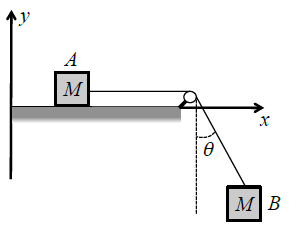
\includegraphics[scale=1]{classica-img/pendulo3.png}
\end{figure}


a) Encontre a aceleração comum dos corpos, se o ângulo $\theta$ é mantido constante e igual a zero e a massa da corda é desprezível.

\resposta

b) Considere agora o movimento mais geral em que o ângulo $\theta$ também pode variar. Suponha que $\theta$ é sempre menor que $\pi/2$ e que o corpo $B$ nunca toca na mesa. Escreva a Lagrangiana do sistema e as equações de movimento (não tente resolver as equações). Mostre que recuperamos o resultado do item (a) se fizermos $\theta = 0$.

\resposta

c) Suponha agora que $\theta$ é novamente mantido constante e igual a zero, mas a corda tem massa não desprezível $m$. Escreva a Lagrangiana do sistema e as equações de movimento. Não é necessário resolver as equações.

\resposta



\item Um disco de raio $R$ é composto por duas metades cada uma com densidades superficiais de massa respectivas de $1\rho$ e de $2\rho$.

\begin{figure}[H]
\centering
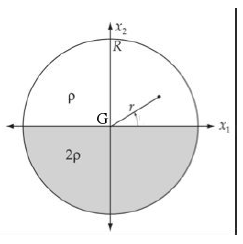
\includegraphics[scale=1]{classica-img/discoraio.png}
\end{figure}


a) Qual é o momento de inércia em relação ao eixo (perpendicular ao plano do disco) que passa pelo seu centro geométrico $G$?

\resposta

b) Encontre as coordenadas $x_{1}$ e $x_{2}$ do centro de massa do disco.

\resposta

c) Qual é o momento de inércia em relação ao eixo (perpendicular ao plano do disco) que passa pelo seu centro de massa?

\resposta

d) Considere o movimento em linha reta do disco sobre um plano horizontal perpendicular ao plano do disco, sem deslizar. Encontre $\lambda(\theta)$, implicitamente definido por
$$
v(t) = \lambda(\theta) R \frac{d\theta}{dt},
$$
onde $\theta$ é o ângulo entre o eixo vertical e a reta que passa pelo centro geométrico e o centro de massa (veja a figura), $v(t)$ é o módulo da velocidade do centro de massa, e $d\theta/dt$ é o módulo da velocidade de rotação do disco.
\begin{figure}[H]
\centering
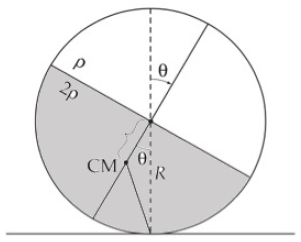
\includegraphics[scale=1]{classica-img/discoraio2.png}
\end{figure}

\resposta


\item Considere um objeto de massa $M$ que se desloca sob ação de uma força central do tipo coulombiana modificada por uma força proporcional ao inverso de $r^{3}$,
$$
F(r) = - \frac{k}{r^{2}} - \frac{q}{r^{3}},
$$
onde $r$ é a coordenada radial, e $k$ e $q$ são constantes positivas. Considere que a energia total do sistema é descrita por
$$
E = \frac{M}{2} \dot{r}^{2} + \frac{M}{2} r^{2} \dot{\theta}^{2} - \frac{k}{r} - \frac{q}{2r^{2}},
$$
e que o momento angular, do sistema é dado por $L = M r^{2} \dot{\theta}$.

a) Para o caso em que o objeto descreva uma órbita circular (de equilíbrio) encontre o raio da órbita em função dos parâmetros $k$, $q$, $M$ e $L$, do sistema.

\resposta

b) Para as mesmas condições do item (a), encontre a energia total, $E$, em função dos parâmetros
k, q, M e L, do sistema.

\resposta

c) Ao identificar o potencial efetivo para o movimento radial como
$$
V_{ef}(r) = \frac{L^{2}}{2mr^{2}} - \frac{k}{r} - \frac{q}{2r^{2}},
$$
verifique sob quais condições sobre as constantes $q$, $L$ e $M$, a coordenada radial da órbita circular obedece uma configuração de equilíbrio estável.

\resposta

d) No caso da coordenada radial da partícula se deslocar da condição de equilíbrio (estável) e passar a oscilar de forma aproximadamente harmônica (em torno do raio da órbita circular), encontre a relação entre o período de oscilação radial e o período de revolução (movimento angular) em função das constantes $q$, $M$ e $L$.

\resposta


\item Uma esfera de bronze sólida de massa $m$ e raio $r$ rola sem deslizar ao longo de um plano inclinado após ser solta do repouso de uma altura $h$. O momento de inércia da esfera em relação a um eixo que passa pelo seu centro é $I = 2mr^{2}/5$ e a aceleração da gravidade é $g$. O plano inclinado forma um ângulo $\theta$ com a horizontal, como mostra a figura.

\begin{figure}[H]
\centering
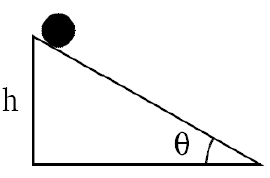
\includegraphics[scale=1]{classica-img/inclinado2.png}
\end{figure}


a) Há atrito entre a esfera e o plano inclinado? Como você chegou a essa conclusão?

\resposta Sim, pois a única força capaz de gerar o torque para que a esfera role sem deslizar é o atrito.

b) Há conservação de energia mecânica? Justifique sua resposta levando em consideração o respondido no item (a).

\resposta Sim, pois o atrito é estático e não realiza trabalho, uma vez que a velocidade do ponto de contato entre a esfera e o plano inclinado é nula (rolamento sem deslizamento).

c) Utilizando considerações de energia, determine a velocidade com que a esfera atinge a base do plano inclinado.

\resposta Tomando a base do plano como o zero de energia potencial gravitacional, a energia mecânica inicial é apenas potencial gravitacional, dada por $E_{i} = mgh$. Na base do plano inclinado, a energia mecânica é puramente cinética, dada pela energia cinética de translação do centro de massa (CM) mais a energia de rotação em torno do CM, ou seja, $E_{f} = mv^{2}/2 + I \omega^{2}/2$, onde $v$ e $\omega$ são, respectivamente, as velocidades de translação do CM e angular na base do plano. Por conservação de energia mecânica,
%
\begin{equation}
  mgh = \frac{1}{2} m v^{2} + \frac{1}{2} I \omega^{2} .
\end{equation}
%
Como há rolamento sem deslizamento, a velocidade de translação do CM e a velocidade de rotação satisfazem $v = \omega r$. Substituindo na Eq. (1) e usando a expressão para o momento de inércia dada no enunciado obtemos
%
\begin{equation}
  v = \sqrt{\frac{10}{7} gh }  .
\end{equation}
%


d) Obtenha a velocidade na base do plano inclinado já calculada no item (c) utilizando agora considerações de dinâmica (ou seja, aplicando a segunda lei de Newton).

\resposta Definimos um sistema de coordenadas com um eixo $x$ paralelo ao plano inclinado e apontando para a base do plano e um eixo $y$ perpendicular ao plano e apontando para cima do plano. A força resultante no eixo $y$ é nula. No eixo $x$, usando a segunda lei de Newton,
%
\begin{equation}\label{eq2}
  mg \sin \theta - f_{at} = ma ,
\end{equation}
%
onde $f_{at}$ é a força de atrito e $a$ a aceleração do CM. Para o movimento de rotação
%
\begin{equation}\label{eq3}
  \tau  = f_{at} r = I \alpha ,
\end{equation}
%
onde $\tau$ é o torque em relação a um eixo que passa pelo CM da esfera e $\alpha$ é sua aceleração angular. Derivando em relação ao tempo a expressão do item anterior, $v = \omega r$, obtemos $a = \alpha r$. Levando esta última relação e a Eq. (\ref{eq2}) na Eq. (\ref{eq3}) obtemos
\begin{equation}
  (mg \sin \theta - ma) r = \frac{2}{5} m r^{2} \frac{a}{r} ,
\end{equation}
%
donde
%
\begin{equation}\label{eq4}
  a = \frac{5}{7} g \sin \theta .
\end{equation}
%
Dado que $a$ é constante, podemos usar a seguinte relação, válida para um movimento uniformemente acelerado,
%
\begin{equation}\label{eq5}
\begin{array}{ccc}
  v^{2} & = & v_{o}^{2} 2 a \Delta x \\
        & = & 2ah / \sin \theta ,
\end{array}
\end{equation}
%
onde $v_{o} = 0$ é a velocidade no instante inicial e $\Delta x = h/\sin \theta$ o deslocamento no eixo $x$. Levando a Eq. (\ref{eq4}) na Eq. (\ref{eq5})
%
\begin{equation}
  v = \sqrt{\frac{10}{7} gh } ,
\end{equation}
%
que coincide com o resultado já encontrado no item (c).




\item Considere uma massa $m$ presa à extremidade de uma haste inextensível de massa desprezível e comprimento $l$. A outra extremidade da haste está presa a um ponto fixo e o sistema haste-massa move-se em um plano vertical num local onde a aceleração da gravidade é $g$.


a) Escreva a Lagrangiana do sistema.

\resposta Utilizaremos como coordenada generalizada o ângulo $\theta$ que a haste faz com a vertical. O módulo da velocidade da partícula é dado por $v = l \dot{\theta}$, de modo que sua energia cinética é
%
\begin{equation}
  T = \frac{m(l \dot{\theta})^{2}}{2} .
\end{equation}
%
A altura na vertical, em relação à posição em que $\theta = 0$, é dada por $h = l - l \cos \theta$. Segue que a energia potencial gravitacional é
%
\begin{equation}
  V = mgl(1 - \cos \theta)
\end{equation}
%
Finalmente, a Lagrangiana do sistema é
%
\begin{equation}\label{eq6}
  L = T - V = \frac{ml^{2} \dot{\theta}^{2}}{2} - mgl(1 - \cos \theta)
\end{equation}
%


b) Obtenha a equação de movimento que descreve o sistema.

\resposta A equação de movimento é obtida a partir da equação de Euler-Lagrange
%
\begin{equation}
  \frac{d}{dt} \left( \frac{\partial L}{\partial \dot{\theta}}  \right) - \frac{\partial L}{\partial \theta} = 0 .
\end{equation}
%
Utilizando a Eq. (\ref{eq6}) na equação acima, temos
\begin{equation}
  \ddot{\theta} = - \frac{g}{l} \sin \theta .
\end{equation}

c) Determine os pontos de equilíbrio do sistema e classifique-os quanto à estabilidade, justificando suas respostas.

\resposta Nos pontos de equilíbrio, $dV / d\theta = 0$, o que nos dá $\sin \theta = 0$, ou seja, os pontos procurados são
$$
\theta = 0 \ \ \ \mbox{e} \ \ \ \theta = \pi .
$$
Para avaliar a estabilidade dos pontos de equilíbrio, analisamos o sinal de
\begin{equation}
  \frac{d^{2}V}{d\theta^{2}} = mgl \cos \theta .
\end{equation}
%
Para $\theta = 0$, a expressão acima tem valor positivo (mínimo de $V$ ), caracterizando um equilíbrio estável, enquanto que para $\theta = \pi$, o sinal é negativo (máximo de $V$ ), correspondendo a um ponto de equilíbrio instável.

d) Encontre a frequência de pequenas oscilações em torno do ponto de equilíbrio estável

\resposta Para pequenas oscilações em torno de $\theta = 0$, podemos aproximar $\sin \theta \approx \theta$. A equação de movimento fica
%
\begin{equation}
  \ddot{\theta} = - \frac{g}{l} \theta ,
\end{equation}
%
cuja solução geral é, por inspeção,
\begin{equation}
  \theta (t) = A \sin (\omega t + \delta) ,
\end{equation}
%
onde $A$ e $\delta$ são constantes arbitrárias determinadas pelas condições iniciais e
%
\begin{equation}
  \omega = \sqrt{g/l} , 
\end{equation}
%
que é a frequência (angular) procurada. Alternativamente, pode-se comparar a Eq. (\ref{eq2}) com a equação de movimento de um oscilador harmônico simples uni-dimensional de frequência (angular) $\omega$,
%
\begin{equation}
  \ddot{x} + \omega^{2} x = 0
\end{equation}
%
e inferir que no caso em questão teremos $\omega = \sqrt{g/l}$




\item É possível construir armadilhas capazes de confinar íons de massa $m$ e carga $q$. Em particular, a armadilha pode restringir o movimento dos íons a apenas uma dada direção espacial, $x$. Assim, considere dois íons de cálcio uma vez ionizado ($Ca^{+}$), submetidos a um potencial confinante externo harmônico $U(x) = m\omega^{2}x^{2}/2$. Esses íons interagem adicionalmente através da repulsão coulombiana,
$$
F_{C} = \frac{e^{2}}{ \left( x^{1} - x^{2} \right)^{2} }
$$
onde $x_{1}$ e $x_{2}$ são as posições dos íons de cálcio e, por simplicidade, foi definido: $e^{2} = q^{2} / (4\pi \epsilon_{0})$.
\begin{figure}[H]
\centering
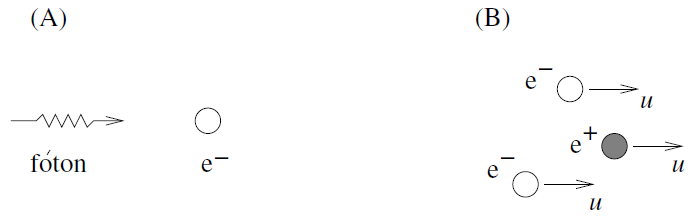
\includegraphics[scale=1]{classica-img/particula.png}
\end{figure}
A figura acima define um sistema de coordenadas conveniente e representa os íons na posição de equilíbrio em que $-x_{1} = x_{2} = x_{0}$. O objetivo deste problema é estudar os modos normais dessa cadeia unidimensional constituida pelos dois íons de cálcio.


a) Obtenha a posição de equilibrio $x_{0}$ em termos de $e$, $m$ e $\omega$.

\resposta


b) Escreva as equações de Newton para o movimento de cada íon e obtenha a frequência de oscilação do sistema quando a separação entre os íons for constante. Este é o primeiro modo normal de oscilação dessa cadeia.

\resposta

c) O segundo modo normal corresponde a um movimento antissimétrico dos íons, em cujo caso o centro de massa está parado em $x = 0$. Obtenha esse segundo modo normal no limite de pequenas oscilações. Obtenha a razão entre as frequências dos dois modos normais de oscilação do sistema.

\resposta

d) As figuras a) e b) abaixo representam os modos normais de oscilação desse sistema de dois íons. Identifique o primeiro e o segundo modo normal obtidos, respectivamente, nos itens (b) e (c) acima. Qual deles tem menor energia?

\begin{figure}[H]
\centering
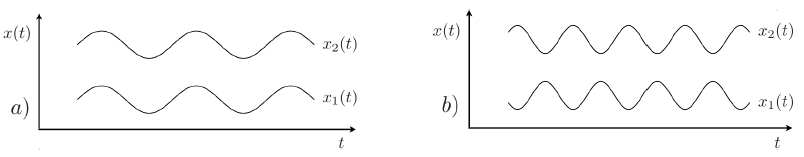
\includegraphics[scale=0.7]{classica-img/ondas.png}
\end{figure}

\resposta

\item Um satélite artificial de massa $m$ está em órbita elíptica em torno da Terra. Admita que a Terra seja uma esfera de densidade uniforme com raio $R$ e massa $M$, e denote por $G$ a constante de gravitação universal. Considere conhecidos $d$ e $D$, as distâncias entre o centro da Terra e o satélite nos pontos de menor e maior afastamento, respectivamente. Uma partícula de massa $m_{0}$ menor do que $m$, choca-se centralmente e de forma completamente inelástica com o satélite no ponto de menor afastamento da Terra. No instante da colisão, o satélite e a partícula tinham velocidades iguais em módulo, mas com sentidos opostos.


a) Obtenha a velocidade $v_{S}$ do sistema satélite-partícula \textit{imediatamente} após a colisão em termos de $v_{p}$, a velocidade no ponto de menor afastamento.

\resposta

b) Expresse o momento angular do satélite nos pontos de mínimo e máximo afastamento em termos de $v_{p}$ e de $v_{a}$ (a velocidade no ponto de maior afastamento), respectivamente, antes da colisão.

\resposta

c) Obtenha a velocidade $v_{p}$, antes da colisão, em termos de $M$, $d$, $D$ e $G$.
d) Obtenha a energia $E_{S}$ e o momento angular $L_{S}$ do sistema satélite-partícula, depois da colisão, em termos de $m_{0}$ e das grandezas que caracterizam o movimento do satélite antes da colisão.

\resposta


\item Uma partícula de massa $m$ está submetida a uma força central conservativa cuja energia potencial é dada por $U(r) = k \left( r^{2} - a^{2} \right)e^{-b r^{2}}$, em que $r$ é a coordenada radial esférica, e $k$, $a$ e $b$ são constantes reais e positivas.


a) Determine as unidades das constante $k$, $a$ e $b$ no SI (Sistema Internacional de Unidades).

\resposta

b) Esboce um gráfico da função $U(r)$, determinando seus pontos de máximo e mínimo em função dos parâmetros dados.

\resposta

c) Determine as faixas de energia $E$ da partícula para as quais (i) a partícula está em órbitas ligadas e (ii) não ligadas. (iii) Determine as condições, se existem, para a existência de órbitas com raio constante.

\resposta

d) Determine a força que age sobre a partícula, diga quais as situações de equilíbrio, se existirem, e, em caso afirmativo determine a frequência de oscilação da partícula para movimentos radiais próximos do(s) ponto(s) de equilíbrio estável.

\resposta




\item Uma partícula de massa $m$ está confinada sobre uma superfície esférica de raio fixo $a$, e nenhuma força externa age sobre a mesma.


a) Determine a lagrangiana da partícula usando coordenadas apropriadas no espaço tridimensional $( \mathbb{R}^{3} )$ e estabeleça a equação de vínculo.

\resposta

b) Usando o método dos multiplicadores de Lagrange, encontre as equações de movimento e determine a força de vínculo, i.e., determine o multiplicador de Lagrange e interprete o resultado.

\resposta

c) Estabeleça as constantes do movimento da partícula.

\resposta

d) Supondo, agora, que o raio da esfera varia no tempo com a função $a(t) = a_{0} (1 + cos \omega t)$, com $a_{0}$ e $\omega$ constantes, determine as constantes de movimento da partícula.

\resposta


\item Duas partículas, $A$ e $B$, de massas $m$ e $M$ ($m \neq M$), respectivamente, estão conectadas às extremidades de um fio inextensível de comprimento $\ell$ e de massa desprezível que passa por um orifício em uma mesa horizontal, como mostrado na figura abaixo. A partícula $A$ move-se sem atrito sobre a mesa enquanto a outra o faz verticalmente sob a ação conjunta da gravidade, de aceleração $\vec{g}$, e da tração do fio (desconsidere também o atrito entre o fio e o orifício).


a) Supondo que a posição inicial de $A$ seja $r = r_{0}$, que velocidade inicial deve ser conferida a ela para que $B$ permaneça em repouso abaixo da superfície da mesa?

\resposta

b) Obtenha as equações do movimento, admitindo que a lagrangiana que descreve um movimento arbitrário desse sistema é dada por
$$
\mathcal{L}=\frac{1}{2}(m+M) \dot{r}^{2}+\frac{1}{2} m r^{2} \dot{\theta}^{2}-M g(r-\ell).
$$

\resposta

c) Obtenha as grandezas conservadas e dê o significado de cada uma delas.

\resposta

d) Se $B$ for ligeiramente e verticalmente deslocada da sua posição, ocorrerão pequenas oscilações no sistema. Obtenha o período dessas oscilações em termos do raio de equilíbrio $r_{eq}$ e das demais grandezas que caracterizam o sistema ($m$, $M$ e $g$).

\begin{figure}[H]
\centering
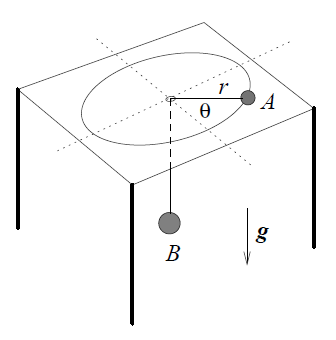
\includegraphics[scale=0.7]{classica-img/mesa.png}
\end{figure}

\resposta



\item Uma partícula de massa $m$ está sujeita ao potencial unidimensional

$$
V(x)=\frac{1}{2} k x^{2}-\frac{k}{4 a^{2}} x^{4}
$$

\begin{figure}[H]
\centering
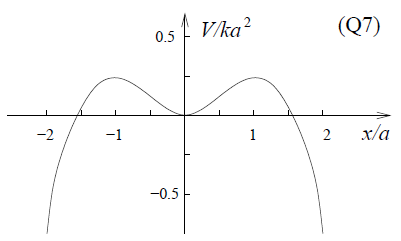
\includegraphics[scale=0.7]{classica-img/pot.png}
\end{figure}
mostrado na figura acima, onde $k$ e $a$ são constantes positivas.


a) Determine a força $F(x)$ e obtenha os pontos de equilíbrio, determinando sua natureza.

\resposta

b) Calcule o período das pequenas oscilações que ocorrem em torno do ponto de equílibrio estável.

\resposta

c) Admita que a partícula esteja em repouso no ponto $x = 0$ e que receba um impulso que lhe confere, instantaneamente, uma velocidade de módulo $v$ na direção de $x$ positivo. Discuta o que ocorre nos seguintes casos: $0<v \leq a \sqrt{k / 2 m} $ e $ v>a \sqrt{k / 2 m}$.

\resposta

d) Esboce o diagrama de fase do sistema ($\dot{x}$ versus $x$ para energia constante) para os diversos tipos de movimento. Indique claramente a curva que corresponde à transição de movimento periódico para não periódico, bem como o valor da energia correspondente.

\resposta




\item Um pêndulo simples é constituído por uma partícula de massa $m$ suspensa por um fio inextensível de comprimento $a$ e massa desprezível. Seu ponto de suspensão é conectado a um suporte que se movimenta horizontalmente sem atrito como mostrado na figura.

\begin{figure}[H]
\centering
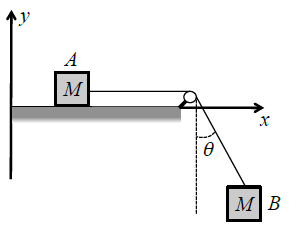
\includegraphics[scale=0.7]{classica-img/pendulo3.png}
\end{figure}

Suponha que o suporte seja muito pequeno e que o pêndulo se movimente apenas no plano vertical. Usando como coordenadas generalizadas $x$ e $\theta$, onde $x$ é a posição horizontal do suporte e $\theta$ o deslocamento angular do pêndulo, conforme se vê na figura, o movimento do sistema é descrito pela lagrangiana:

$$
\mathcal{L}=\frac{m}{2} \dot{x}^{2}+\frac{m}{2}\left(a^{2} \dot{\theta}^{2}+2 a \dot{x} \dot{\theta} \cos \theta\right)+m g a \cos \theta
$$


a) Obtenha a equação de movimento para a coordenada $\theta$.

\resposta

b) Admitindo que os deslocamentos angulares sejam pequenos e que o suporte esteja sujeito a um movimento harmônico forçado de frequência $\omega$, isto é, descrito por $x(t) = x_{0} cos \omega t$, obtenha a solução geral $\theta(t)$ da equação do movimento para a coordenada $\theta$.

\resposta

c) No caso do item anterior, obtenha a frequência de ressonância $\omega R$.

\resposta

d) Escreva a solução geral para $\theta(t)$, quando as condições iniciais forem $\theta(0) = 0$ e $\dot{\theta}(0) = 0$ e o suporte movimentar-se com frequência $\omega < \omega_{R}$.



\item Um átomo de trítio pode ser descrito classicamente como um núcleo com carga elétrica $+e$, composto por um próton e dois nêutrons, circundado por um elétron orbital de carga $-e$, o qual percorre uma órbita circular de raio $r_{0}$. Em um processo conhecido como decaimento beta, o núcleo de trítio se transforma em um núcleo de hélio, composto por dois prótons e um nêutron, emitindo um par de partículas que rapidamente escapa do sistema atômico. Como
consequência desse processo, o átomo de hélio fica ionizado uma vez, e o elétron orbital passa subitamente para uma nova situação, orbitando agora em torno de um núcleo de carga $+2e$.


a) Supondo que o par de partículas que escapa do átomo tenha momento linear total de módulo $p$, obtenha a velocidade de recuo do átomo de hélio de massa $M$.

\resposta

b) Obtenha a energia $E_{a}$ do elétron orbital antes do decaimento beta.

\resposta

c) Calcule a energia $E_{d}$ do elétron orbital depois do decaimento beta e obtenha a razão $\rho = E_{a}/E_{d}$.

\resposta

d) Determine o momento angular total do elétron em função de $r_{0}$ e da massa $m$ do elétron. Calcule a maior e a menor distância entre o elétron e o núcleo na nova órbita em termos de $r_{0}$.

\resposta


\item Um equilibrista de massa $m$ está inicialmente parado na extremidade de uma barra larga, horizontal, homogênea, de comprimento $D$ e massa $M = 3m$. A barra gira em torno de um eixo vertical que passa pelo seu centro. O equilibrista começa então a caminhar sobre a barra, em direção ao eixo de rotação, com velocidade constante. Considere o período inicial de rotação do sistema igual a $T_{0}$.

a) Determine o torque das forças que atuam sobre o equilibrista em relação ao centro da barra.

\resposta

b) Determine o momento angular do sistema quando o equilibrista atinge o centro da barra. Determine o período de rotação do sistema nessa situação.

\resposta

c) Determine as energias nas posições inicial e final do sistema. Nesse movimento, a energia do sistema variou?

Considere o equilibrista como uma massa puntiforme.

Dado: $I_{CM}(barra) = \frac{1}{12} MD^{2}$

\resposta




\item Uma partícula de massa $m$ se encontra no interior de um cano oco, liso, estreito e longo que gira num plano horizontal com velocidade angular $\omega$ constante. O eixo fixo de rotação passa por uma das extremidades do cano, como mostra a figura.

\begin{figure}[H]
\centering
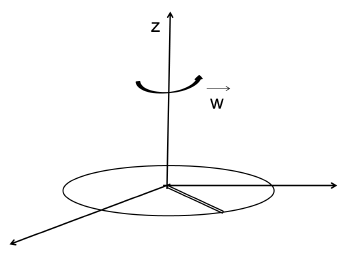
\includegraphics[scale=0.8]{classica-img/angular.png}
\end{figure}


a) Escreva a Lagrangiana da partícula.

\resposta

b) Obtenha as equações de Lagrange do movimento da partícula.

\resposta

c) Determine o movimento da partícula, considerando que inicialmente ela é lançada do centro de rotação com velocidade $\vec{v}_{0}$.

\resposta

d) Obtenha a função Hamiltoniana ($H$) do movimento dessa partícula e as equações de Hamilton do movimento.

\resposta

e) Dentre as grandezas físicas $H$ e $E$ (energia), quais são conservadas? Justifique sua resposta.

\resposta





\item Uma partícula de massa $m$ move-se com velocidade $\vec{v}_{1}$ no semi-plano superior até ser desviada ao atingir o semi-plano inferior, onde passa a se propagar com velocidade $\vec{v}_{2}$, conforme ilustrado na figura abaixo. Observa-se experimentalmente as seguintes características: i) a partícula passa do meio 1 ao meio 2 desde que $v_{1} > v_{min}$; ii) a partícula se move de modo retilíneo e uniforme em cada um dos semi-planos; iii) o ângulo de saída $\theta_{2}$ é diferente do ângulo de entrada $\theta_{1}$, o que nos faz presumir que em cada meio a partícula esteja sob ação de diferentes
potenciais $U_{1}$ e $U_{2}$.

\begin{figure}[H]
\centering
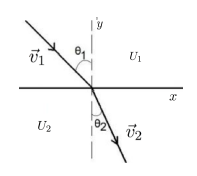
\includegraphics[scale=0.8]{classica-img/refracao.png}
\end{figure}


a) Com base no experimento, esboce o gráfico do potencial $U$ em função de $y$ para $x$ fixo (justificando o gráfico).

\resposta

b) Determine $v_{2}$ em termos de $v_{1}$, de $m$ e dos potenciais $U_{1}$ e $U_{2}$. Qual é a velocidade $v_{min}$ acima da qual observa-se a passagem da partícula do meio 1 para o meio 2?
\item(c) Determine o índice de refração $sen\ \theta_{1} / sen\ \theta_{2}$ em termos de $m$, $v_{1}$ e dos potenciais em cada
meio.

\resposta


\item Uma partícula de massa $m$ desenvolve movimento unidimensional sob ação do potencial abaixo ($c$ é uma constante)

$$
U(x) = \frac{1}{2} x^{4} - c x^{2}.
$$


a) Esboce os gráficos de $U(x)$ e dos respectivos espaços de fase ($\dot{x}$ versus $x$ para todas as energias possíveis) nos seguintes casos : i) $c > 0$, ii) $c = 0$ e iii) $c < 0$.

\resposta

b) Por meio da energia total $E$, identifique todos os movimentos periódicos possíveis e seus respectivos pontos de inversão (onde a velocidade é nula) para cada um dos casos do item (a).

\resposta

c) Determine a dependência do período de oscilações com a energia total $E$ para $c = 0$.

\resposta



\item Duas esferas ocas, ambas de massa $M$ e raio $R$, que estão girando em torno do centro de massa ($CM$) do sistema com um período inicial $T_{0}$, são mantidas distantes $d_{0} = 8R$ uma da outra por um fio ideal que passa pelos respectivos centros, conforme ilustra a figura abaixo.
\begin{figure}[H]
\centering
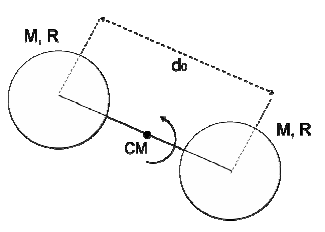
\includegraphics[scale=0.8]{classica-img/rotacional.png}
\end{figure}
Num dado instante um motor, colocado dentro de uma das esferas, começa a enrolar o fio lentamente, aproximando uma esfera da outra. Considere que o momento de inércia do motor seja desprezível quando comparado ao das esferas. Desconsidere efeitos da gravidade e expresse todos os seus resultados em termos de $M$, $R$ e $T_{0}$. Dado: o momento de inércia da casca esférica em relação a um eixo que passa pelo seu centro é $\frac{2}{3} MR^{2}$.

a) Determine o momento angular desse sistema em relação ao seu centro de massa, antes do motor ser ligado.

\resposta

b) Calcule a velocidade angular de rotação, $\omega_{f}$ , no instante em que uma esfera encosta-se à outra.

\resposta

c) Calcule a variação da energia cinética do sistema até esse instante.

\resposta

d) Qual foi o trabalho realizado pelo motor para fazer com que as esferas se encostem?

\resposta


\item Um pêndulo simples consiste de uma massa m pendurada a partir de um ponto fixo por uma barra estreita de massa desprezível, inextensível, de comprimento $\ell$. Seja $g$ a aceleração da gravidade local e $\theta$ o ângulo entre o pêndulo e a direção vertical. No que segue, faça sempre a aproximação de pequenos ângulos.

a) Escreva a equação de movimento desprezando o atrito. Obtenha a frequência natural $\omega$ do pêndulo.

\resposta

b) Determine $\theta(t)$ para as seguintes condições iniciais: $\theta(0)=0$ e $\frac{d \theta}{d t}(0)=\Omega$.

\resposta

c) Escreva a equação do movimento do pêndulo na presença de uma força de atrito viscoso dada por $F_{R}=2 m \sqrt{g l} \frac{d \theta}{d t}$.

\resposta

d) Na situação do item (c), determine $\theta (t)$ para as seguintes condições iniciais: $\theta(0) = \theta_{0}$ e $\frac{d\theta}{dt} (0) = 0$.

\resposta


\item Um corpo celeste de massa $m$ se aproxima do Sol (massa $M >> m$) seguindo uma trajetória hiperbólica e quando está a uma distância $r_{0}$ dele, a sua velocidade é $v_{0}$ e faz um ângulo de $30º$ com o raio vetor ao Sol.

a) Calcule o momento angular $L$ e a energia $E$ desse corpo celeste.

\resposta

b) Determine a distância $r_{p}$ de máxima aproximação do corpo celeste ao Sol, expressando o seu resultado em termos de $L$ e $E$.

\resposta

c) Quando o corpo celeste atinge a distância $r_{p}$ de máxima aproximação, sofre um choque com um pequeno asteróide de tal maneira que sua massa não varia, porém ele passa a descrever órbita circular de raio $r_{p}$ no mesmo plano da órbita anterior. Calcule a nova energia e o novo momento angular do corpo celeste após a colisão, expressando o seu resultado em termos de $r_{p}$.

\resposta


\item Uma bola de massa $m = 450 g$ está presa a uma mola cuja energia potencial em função da elongação $x$ está mostrada na figura abaixo (linha sólida). Expresse as respostas no SI.

a) Determine a constante elástica da mola, para pequenos deslocamentos.

\resposta

b) Esboce um gráfico da força que atua sobre essa bola em função da elongação da mola. Sabendo que o movimento da bola é unidimensional e sua elongação máxima é de 3 $cm$:

\resposta

c) determine sua velocidade máxima;

\resposta

d) determine a energia cinética da bola nesse movimento para a elongação da mola $x = - 2 cm$;

\resposta

e) Determine a posição ($x < 0$) em que a bola deve ser solta a partir do repouso para atingir o ponto $x = 5 \ cm$ com velocidade nula.

\begin{figure}[H]
\centering
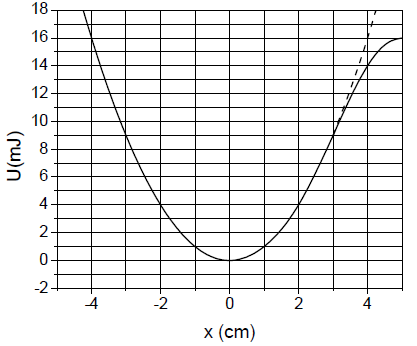
\includegraphics[scale=0.8]{classica-img/grafico.png}
\end{figure}

\resposta

\item Considere um corpo de massa $M$ de seção transversal circular de raio $R$ que rola sem deslizamento sobre um plano que possui um ângulo de inclinação $\mu$ em relação à horizontal, conforme mostra a figura abaixo. O coeficiente de atrito estático entre o corpo e o plano é $\mu_{e}$. O momento
de inércia do corpo em relação a um eixo passando pelo ponto $O$ é $I$ e a aceleração da gravidade é $g$.


a) Desenhe o diagrama de forças para o corpo. Escreva a equação que relaciona a velocidade angular, $\dot{\phi}$, de rolamento do corpo e a velocidade de translação, $\dot{x}$, que caracteriza um rolamento sem deslizamento.

\resposta

b) Determine a aceleração $\ddot{x}$, associada à translação do corpo ao longo do plano inclinado, em termos dos parâmetros que constam no enunciado.

\resposta

c) Assuma que o corpo inicia o seu movimento a partir do repouso na origem do sistema de coordenadas cartesianas indicado na figura. Calcule a energia mecânica no início e no final do movimento. A energia mecânica do sistema é conservada?

\resposta

d) Calcule o momento de inércia $I$ considerando que o corpo seja (i) um anel e (ii) um disco. Assuma que as massas dos corpos estão uniformemente distribuídas. Suponha agora que o ângulo $\mu$ possa ser variado. A partir de qual $\mu$ cessa o movimento de rolamento puro e o corpo começa a deslizar, nos casos (i) e (ii) acima? Deixe a resposta em termos de $\mu_{e}$.

\resposta


\item Considere o pêndulo invertido da figura abaixo, composto por uma barra de massa M e momento de inércia $I_{0}$ em relação ao seu centro de massa, cujas coordenadas são ($X,Y$). A barra pode girar livremente no plano $xy$ em torno de um eixo de rotação que passa pela posição ($x_{p},y_{p}$), a uma distância $\ell$ do centro de massa. A aceleração da gravidade é $g$.
\begin{figure}[H]
\centering
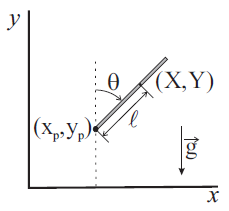
\includegraphics[scale=0.8]{classica-img/pendulo5.png}
\end{figure}

a) Escreva as equações para a energia cinética e potencial do sistema em termos de $X$, $Y$ e $\mu$. Para os itens (b), (c) e (d) assuma que um agente externo faz o eixo de rotação oscilar horizontalmente com frequência angular $\omega$, ou seja, tem-se $y_{p}(t) = 0$ e $x_{p}(t) = A cos(\omega t)$.

\resposta

b) Escreva a lagrangiana do sistema em termos da coordenada generalizada $\theta$.

\resposta

c) Escreva a equação de movimento para a lagrangiana do item (b).

\resposta

d) Considere que o sistema executa pequenas oscilações ($\theta$ pequeno). Mostre que neste caso, $\theta(t) = \alpha cos(\omega t) + \beta sen( \omega t)$ é uma solução para o problema. Determine $\alpha$ e $\beta$.

\resposta


\item Uma bala de massa $m$ é disparada com velocidade $v$ contra um disco homogêneo de massa $M$ e raio $R$, inicialmente parado, que se encontra deitado sobre uma superfície horizontal lisa sem atrito. Suponha que a bala atinja o disco como indicado na figura e fique retida na superfície do disco. Considere que o centro de massa do sistema (disco + bala) após a colisão coincide com o centro do disco. $Dado$: $I_{disco}^{CM} = \frac{1}{2} M R^{2}$.

a) Qual é a velocidade do centro do disco após a colisão?

\resposta

b) Qual é a velocidade angular dos sistema (disco + bala) após a colisão?

\resposta

c) Qual é a variação de energia dos sistema devido à colisão?

\begin{figure}[H]
\centering
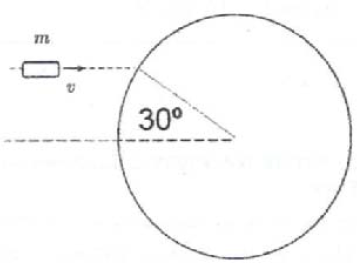
\includegraphics[scale=0.7]{classica-img/angular2.png}
\end{figure}

\resposta

\item Uma partícula de massa $m$ sob a ação da gravidade $g$ constante está vinculada a se mover no interior da superfície de um cone invertido cuja geratriz forma um ângulo $\alpha$ com o eixo do cone. O vértice do cone está na origem e seu eixo ao longo da direção vertical. O atrito pode ser desprezado.

a) Determine a energia cinética e a energia potencial da partícula. \textit{Sugestão: utilize coordenadas esféricas.}

\resposta

b) Escreva a lagrangiana do sistema e obtenha as equações do movimento.

\resposta

c) Há grandezas físicas conservadas no movimento dessa partícula? Se há, diga quais são essas grandezas, argumentando sobre como chegou à conclusão de que são conservadas.

\resposta

d) A partir da definição da hamiltoniana, obtenha sua forma explícita em termos das coordenadas e momentos generalizados, e compare-a com a energia mecânica da partícula.

\resposta

e) Mostre que a partícula, em questão pode executar pequenas oscilações radiais em torno de um raio de equilíbrio $r_{0}$ e determine sua frequência. Compare o valor obtido com a frequência de revolução no movimento circular.

\resposta


\item Uma partícula de massa $m$ colide com uma barra fina e homogênea inicialmente em repouso, de momento de inércia $I = Ml^{2}/12$ relativo ao seu centro de massa, sendo $M$ a sua massa e $\ell$ o seu comprimento. Antes da colisão, a partícula move-se perpendicularmente à barra com velocidade $v_{0}$. A partícula colide elasticamente com a extremidade da barra, conforme ilustra a figura a baixo.
\begin{figure}[H]
\centering
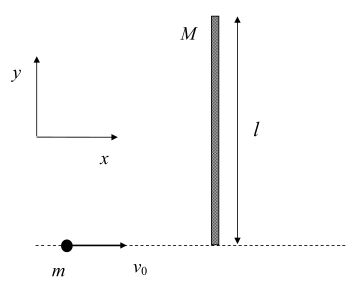
\includegraphics[scale=0.7]{classica-img/colide.png}
\end{figure}

a) Escreva as equações que expressam as grandezas físicas conservadas na colisão.

\resposta

b) Determine o vetor velocidade de translação do centro de massa da barra imediatamente após a colisão.

\resposta

c) Determine o vetor velocidade angular de rotação da barra imediatamente após a colisão.

\resposta

d) Determine o vetor velocidade da partícula imediatamente após a colisão.

\resposta


\item Uma partícula de massa $m$ pode se mover sem atrito num aro de raio $R$, como mostrado na figura abaixo. O aro gira com velocidade angular constante $\omega$ em torno do eixo vertical, como mostra a figura abaixo. Considere a aceleração da gravidade $g$.
\begin{figure}[H]
\centering
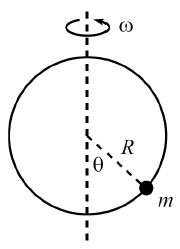
\includegraphics[scale=0.7]{classica-img/particula2.png}
\end{figure}

a) Determine a energia cinética da partícula em função de $\theta$, $\dot{\theta}$, $R$, $m$, e $\omega$.

\resposta

b) Determine a lagrangiana da partícula, adotando energia potencial nula no ponto correspondente a $\theta = 0$.

\resposta

c) Determine a equação de movimento da partícula.

\resposta

d) Determine os pontos de equilíbrio.

\resposta


\item A interação entre dois átomos de massas $m_{1}$ e $m_{2}$, que formam uma molécula, pode ser descrita pelo potencial de Lennard-Jones dado por
$$
V(x) = A \left[ \left( \frac{b}{x} \right)^{12} - 2 \left( \frac{b}{x} \right)^{6} \right]
$$
onde $A$ e $b$ são parâmetros positivos e $x$ a separação interatômica. Trate o problema classicamente e despreze qualquer tipo de rotação da molécula.

a) Determine a posição de equilíbrio em função de $A$ e $b$.

\resposta

b) Calcule a menor energia para dissociar a molécula.

\resposta

c) Mostre que o equilíbrio é estável e calcule a frequência de pequenas oscilações em torno da posição de equilíbrio.

\resposta

d) Desenhe um gráfico do potencial de Lenard-Jones indicando os parâmetros obtidos nos itens (a) e (b).

\resposta


\item Atualmente, a totalidade dos atletas de alto nível de salto em altura utiliza uma técnica para o salto batizada de "Salto Fosbury". Suponha que nesse salto o atleta possa ser aproximado por uma barra rígida de comprimento $\ell$, inclinada por um ângulo $\theta$ e movendo-se com uma velocidade $v_{0}$ para a direita conforme mostra a figura abaixo. No momento do "salto" essa barra começa a girar em torno do ponto \textbf{P}. A barra possui uma massa $m$ homogeneamente distribuída.
\begin{figure}[H]
\centering
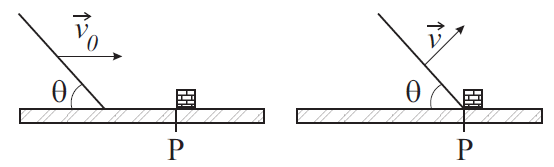
\includegraphics[scale=0.7]{classica-img/massa.png}
\end{figure}

a) Calcule o momento de inércia da barra em relação à sua extremidade.

\resposta

b) A conservação de uma grandeza física permite que a barra obtenha uma componente vertical para a velocidade do seu centro de massa. Qual é essa grandeza física?

\resposta

c) Calcule a componente vertical $\nu_{v}$ da velocidade do seu centro de massa imediatemente após atingir o ponto \textbf{P}.

\resposta

d) Qual é a altura máxima atingida pelo seu centro de massa em relação ao solo.

\resposta


\item Uma barra uniforme de comprimento $L$ e massa $M$ está em equilíbrio numa mesa horizontal sobre a qual pode mover-se sem atrito. Num dado instante a barra recebe um impulso, $J$, de curta duração perpendicular à barra num ponto P da barra tal que $OP = r$, onde  $O$ é o centro de massa da barra.

a) Logo após o impulso, qual é a velocidade do centro de massa da barra?

\resposta

b) Qual é a velocidade angular da barra em torno do centro de massa?

\resposta

c) Qual é a velocidade da extremidade da barra mais afastada do ponto de impacto P?

\resposta

d) Qual é a localização de um ponto $Q$ da barra, para o qual a velocidade instantânea é nula?

\resposta



\item Uma maneira de transferir um foguete de uma órbita circular para outra é fazê-lo percorrer uma órbita elíptica de transferência que tangencia as duas órbitas circulares. Considere que as órbitas da Terra e de Marte são órbitas circulares de raios iguais à $R_{1}$ e $R_{2}$ respectivamente e que um foguete é lançado da Terra até Marte numa órbita elíptica de transferência tal que o seu periélio (distância de maior aproximação) está na órbita de Terra e o seu afélio (distância de maior afastamento) na órbita de Marte.

a) Qual é a velocidade do foguete relativa a Marte quando eles se encontram?

\resposta

b) O que devemos fazer para que o foguete pouse em Marte?

\resposta

c) Qual é o tempo de transferência?

\item[] São conhecidos: $G$: (constante gravitacional) e $M$ (massa do sol).

\resposta

\item Dois patinadores de mesma massa estão sobre a superfície de um lago congelado. Um deles, A, está em repouso, enquanto que o outro, B, se aproxima do primeiro com velocidade $\vec{v}$ e parâmetro de impacto $b$ menor que o comprimento dos braços dos patinadores. No instante em que a distância entre eles é mínima, eles seguram-se pelas mãos.

a) Qual é a velocidade angular de rotação dos patinadores em torno do centro de massa?

\resposta

b) Qual é o tempo mínimo que eles devem permanecer unidos para que o patinador que estava parado, A, saia formando um ângulo de $30°$ com a direção de $\vec{v}$ no sistema de laboratório?

\resposta

c) Qual é a tensão nos braços dos patinadores?

\resposta


\item Duas partículas de massas iguais a $m$ estão ligadas por uma corda inextensível de comprimento $\ell$ e massa desprezível, que passa por um pequeno furo sobre uma mesa horizontal. Uma das partículas se move na superfície da mesa horizontal e a outra ao longo da direção vertical.

a) Tomando para coordenadas generalizadas, as coordenadas polares $\rho$, $\phi$ da partícula que se move no plano da mesa, num sistema de coordenadas cuja origem coincide com o furo na mesa, mostre que a lagrangeana do sistema é igual a:
$$
L = m\dot{\rho}^{2} + \frac{1}{2} m \rho^{2} \dot{\rho}^{2} - mg\rho
$$

\resposta

b) Escreva as equações de Lagrange.

\resposta

c) Mostre que o momento angular em relação do furo da mesa é uma constante do movimento.

\resposta

d) Mostre que é possível haver movimento circular no plano da mesa.
\item[] Calcule o momento angular e a energia do sistema, se a partícula no plano da mesa se move numa órbita circular de raio R.

\resposta


\item Uma partícula de massa $m$ e carga $q$ é lançada verticalmente da superfície terrestre com velocidade $v_{0}$ na direção de uma carga $Q$ de sinal oposto ao da carga $q$, Qq<0, fixa a uma altura h suficientemente pequena para considerarmos $g$ constante. A energia potencial da partícula é igual a, para $0 < z < h$:
$$
U(z) = mgz - \frac{|Qq|}{h-z}
$$

a) Mostre que se $h$ é menor que um valor mínimo $h_{min}$, as cargas sempre se chocam, independente do valor de $v_{0}$.

\resposta

b) Mostre que se $h$ exceder esse valor, as cargas se chocam somente se $v_{0}$ for maior do que um valor mínimo, $v_{min}$.

\resposta

c) Nas condições do item (b), existe um ponto de equilíbrio? Ele é estável?

\resposta


\item O ponto de suspensão de um pêndulo de massa $m$ e comprimento $\ell$ oscila na direção horizontal de acordo com a equação
$$
x_{p} = a \operatorname{cos} \omega t
$$
Considere que o pêndulo se move num plano vertical.

a) Mostre que a lagrangeana do sistema é igual a:
$$
L = \frac{m}{2} (\dot{x}_{p}^{2} + \ell^{2} \dot{\theta}^{2} + 2 \ell \operatorname{cos}(\theta) \dot{x}_{p} \dot{\theta} ) + mgl \operatorname{cos} \theta
$$
onde $\theta$ é o ângulo que a direção do pêndulo faz com a vertical.

\resposta

b) Escreva a equação de Lagrange.

\resposta

c) Interprete a equação de movimento deduzida no item (b) do ponto de vista de um observador fixo no ponto de suspensão do pêndulo. Qual é a origem dos termos desta equação?

\resposta


\item Duas estrelas, de massas $m_{1}$ e $m_{2}$, se movem em órbitas circulares em torno do seu centro de massa, sob a ação da atração gravitacional entre ambas. O centro de massa está em repouso e a distância entre elas é igual a $D$.

a) Calcule os raios das órbitas circulares.

\resposta

b) Faça um gráfico das órbitas. Assinale uma possível posição das estrelas, num dado instante $t$. Considere $m_{1} >  m_{2}$.

\resposta

c) Qual é o período do movimento orbital?

\resposta

d) Que observação astronômica indicaria que um dos constituintes desse sistema binário seja um buraco negro?

\resposta


\item Um astronauta está viajando numa nave que é um disco de massa M e raio R. Por engano ele aciona dois foguetes, que são lançados ao mesmo tempo, tangentes à nave e em direções opostas, com velocidade $v$ e massas $m$. Os pontos de lançamento são diametralmente opostos e a nave inicialmente estava em repouso. Considere $M >> m$.

a) Qual a velocidade angular da nave após o lançamento?

\resposta

b) Que propriedade você usou para responder à pergunta do item $a$?

\resposta

c) O astronauta, para interromper a rotação da nave, lança um jato de combustível de massa igual a $\frac{m}{10}$, tangente à nave. Qual deve ser a velocidade de lançamento?

\resposta

d) Após o lançamento do combustível, a nave fica estacionária? Explique.
\item[] Dado: Momento de inércia do disco em torno do eixo de simetria, perpendicular ao plano do disco, $I = \frac{MR^{2}}{2}$.

\resposta


\item Uma nave espacial tem a forma de um cilindro oco de raio interno $R_{1}$ e raio externo $R_{2}$. A região compreendida entre os raios $R_{1}$ e $R_{2}$ é a região oca, sendo o "teto" da nave a superfície de raio $R_{1}$ e o "solo" a de raio $R_{2}$. A nave está numa região livre de campos gravitacionais, mas o efeito da gravidade pode ser simulado fazendo com que a nave gire com velocidade angular $\omega$ em torno do eixo de simetria do cilindro.

a) Se um objeto de massa $m$ está preso no teto da nave, qual é o seu "peso"?

\resposta

b) Se deixarmos o objeto cair , quais são suas trajetórias, vistas por: um observador  num referencial inercial e um observador num referencial fixo na nave? Responda sem fazer cálculos.

\resposta

c) Quanto tempo ele leva para atingir o "solo"?

\item[] Dados:
\item[] Força centrífuga$ = - m \vec{\omega} \times (\vec{\omega} \times \vec{r})$
\item[] Força de Coriolis$ = -2m (\vec{\omega} \times \vec{v})$

\resposta


\item Uma partícula de massa $m$ se move na superfície de um cilindro de raio $R$ sob a ação da gravidade e de uma força central cuja energia potencial é
$$
U_{cent} = \frac{kr^{2}}{2},
$$
onde $r$ é a distância da partícula ao centro de forças e $k$ é uma constante positiva. O centro de forças está localizado no eixo de simetria do cilindro e esse eixo de simetria está na direção vertical (ver figura abaixo; a aceleração da gravidade tem sentido oposto a $Oz$).
\begin{figure}[H]
\centering
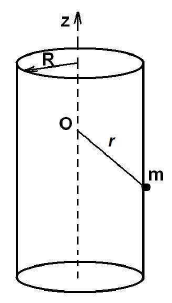
\includegraphics[scale=0.7]{classica-img/cilindro.png}
\end{figure}


a) Mostre que a lagrangeana da partícula em coordenadas cilíndricas num sistema de coordenadas com origem no centro de forças e eixo $Oz$ na direção vertical é dada por:
$$
L  = \frac{m}{2} (R^{2} \dot{\phi}^{2} + \dot{z}^{2} ) - mgz - \frac{k}{2} (z^{2} + R^{2}).
$$

\resposta

b) Escreva as equações de Lagrange.

\resposta

c) É possível haver movimento circular em um plano horizontal? No caso afirmativo, qual é a localização do plano?

\resposta

d) Determine a frequência de pequenas oscilações em torno do movimento circular.

\resposta



\item Decidiu-se colocar em órbita um satélite geoestacionário em duas etapas. Inicialmente o satélite se encontra numa órbita circular de estacionamento, no mesmo plano da órbita geoestacionária. O período da órbita de estacionamento é igual a $\frac{2}{3}T$, onde $T$ é o período de rotação da Terra em torno do seu eixo. Para transferir o satélite para a órbita circular geoestacionária foi decidido fazê-lo através de uma órbita elíptica cujo perigeu (distância de maior aproximação) está na órbita de estacionamento e o apogeu (distância de maior afastamento) na órbita geoestacionária.

a) Qual é a localização do plano das órbitas satélite?

\resposta

b) Determine, em função dos dados abaixo, os raios das órbitas de estacionamento e geoestacionária.

\resposta

c) Qual é o tempo de transferência?

\resposta

d) Discuta como se deve proceder para que o satélite se encontre, no fim da operação, sobre o mediano de Brasília.

\item[] Dados:
\item[] $G =$ constante gravitacional.
\item[] $M =$ massa da Terra.
\item[] $T =$ período de rotação da Terra em torno do seu eixo.
\item[] \textbf{Observação: fornecer as respostas em função dos dados.}

\resposta



\item Um cubo uniforme de aresta $2a$ e massa $M$ desliza com velocidade $v$ sobre uma mesa horizontal quando se choca com uma saliência da mesa, paralela à aresta do cubo, e gruda na saliência, passando a rodar em torno dela.

a) Qual é a velocidade angular do cubo devida ao choque?

\resposta

b) Qual é a perda de energia cinética imediatamente após o choque?

\resposta

c) Determine o valor mínimo de $v$ para que o cubo tombe (caia do outro lado da saliência.)

\item[] Dado:
\item[] Tensor de inércia do cubo num sistema de coordenadas cujo eixo $Oz$ coincide com uma das arestas e a origem está no meio da aresta:

$$
I = \left(
\begin{array}{ccc}
\frac{5}{3} M a^{2} & -Ma^{2} & 0 \\
- M a^{2} & \frac{5}{3} M a^{2} & 0 \\
0 & 0 & \frac{5}{3} M a^{2} \\
\end{array}
\right)
$$



\item Um objeto de massa $M_{1}$ está preso no teto de um elevador de massa $M_{2}$. O elevador está see deslocando para cima pela ação de uma força constante $F$, $F > (M_{1} + M_{2})g$. O objeto de massa $M_{1}$ está preso no teto através de um fio inextensível e está a uma distância $s$ do chão do elevador.

a) Qual é a aceleração do elevador?

\resposta

b) Qual é a tensão no fio inextensível?

\resposta

c) Se o fio quebra repentinamente, qual é a aceleração do elevador? Qual é a aceleração do objeto de massa $M_{1}$?

\resposta

d) Quanto tempo leva para o objeto de massa $M_{1}$ atingir o chão do elevador?

\item[] Dados: $F$, $M_{1}$, $M_{2}$, $g$, $s$.
\item[] Observação: fornecer as respostas em função dos dados.




\item Uma partícula e uma barra podem se mover livremente sobre a superfície lisa de uma mesa horizontal. A barra tem comprimento $D$ e massa igual à massa da partícula, $M$. Inicialmente a barra está em repouso, e a partícula se move com velocidade $v$ perpendicular à barra. Suponha que a partícula colide com a barra e que a colisão é elástica.

a) Descreva os movimentos subsequentes da partícula e da barra quando a partícula colide com a barra no seu centro de massa (ver figura a) abaixo).

\resposta

b) Descreva os movimentos subsequentes da partícula e da barra quando a partícula colide com a barra numa das suas extremidades (ver figura b) abaixo).

\resposta

c) No caso do item (b), determine as velocidades da partícula, $v_{p}$, da barra, $v_{b}$, e a velocidade angular de rotação da barra em torno do seu centro de massa, $w$.

\item[] Momento de inércia da barra relativo a um eixo passando pelo centro de massa e perpendicular à barra: $I = MD^{2}/12$.

\begin{figure}[H]
\centering
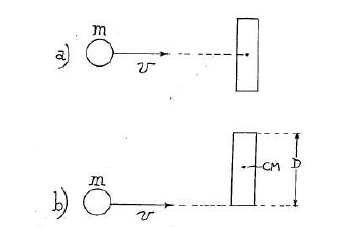
\includegraphics[scale=0.7]{classica-img/barra2.png}
\end{figure}

\resposta


\item Um objeto de massa $m$ desliza num trilho liso mostrado na figura ao lado. Inicialmente o objeto está em repouso, a uma altura $h$ acima do topo do semicírculo $AC$.
\begin{figure}[H]
\centering
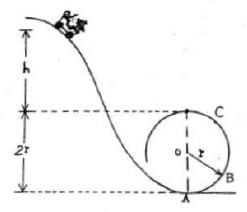
\includegraphics[scale=0.7]{classica-img/trilho.png}
\end{figure}

a) Faça um diagrama das forças que agem no objeto quando ele está no ponto $B$ do semi-círculo. Defina $\theta$ como o ângulo do vetor posição medido em relação à direção $\overline{OA}$. Escreva as equações de movimento nas direções radial e tangencial.

\resposta

b) Qual é a magnitude e direção da força exercida no objeto pelo trilho, quando ele passa no ponto A?

\resposta

c) Mostre que $h \geq r/2$, para que o objeto atinja o ponto C do trilho.

\resposta

d) Para $h < r/2$ o objeto abandona o trilho antes de atingir o ponto C. Mostre que isto ocorre na posição tal que $-3 \operatorname{cos} \theta = 2 + 2h/r$.

\resposta




\item Um plano inclinado de um ângulo $\alpha$ é acelerado horizontalmente. A magnitude da aceleração aumenta gradualmente até que um bloco de massa $m$, originalmente em equilíbrio com respeito ao plano inclinado, começa a subir no plano. O coeficiente de atrito estático entre o bloco e o plano é $\mu = 5/4$.

a) Desenhe um diagrama mostrando as forças que atuam no bloco, pouco antes dele subir no plano, visto de um referencial inercial.

\resposta

b) Ache a aceleração do plano quando o bloco começa a subir.

\resposta

c) Repita o item (a) visto de um referencial não inercial, fixo no plano.
\item[] Dado: $\operatorname{cos} \alpha = 0,8$; $\operatorname{sen} \alpha = 0,6$

\resposta



\item Uma partícula de massa igual a $m$ se move no interior de um cano liso. O cano, por sua vez, gira num plano horizontal com velocidade angular $\omega$ constante em torno de um ponto fixo no cano.

a) Quantos graus de liberdade tem a partícula?

\resposta

b) Considere como coordenada generalizada a posição da partícula ao longo do cano, $s$, com a origem no centro de rotação. Mostre que a lagrangeana do sistema é dada por:
$$
L = \frac{1}{2} m \left( \dot{s}^{2} + \omega^{2} s^{2} \right)
$$

\resposta

c) Escreva a equação de Lagrange. Existe um ponto de equilíbrio? Ele é estável?
d) Determine a força de reação do cano. Do ponto de vista de um observador fixo no cano, qual é a origem da força de reação?

\resposta




\item A massa $m$ de um pêndulo está presa por um fio ideal de comprimento $\ell$ a um ponto de sustentação. Esse ponto se move para a frente e para trás ao longo de um eixo horizontal, de acordo com a equação $x = a \operatorname{cos} \omega t$. Suponha que o pêndulo só oscile no plano vertical que contém o eixo $x$. Considere que a posição do pêndulo seja descrita por um ângulo $\theta$ que o fio faz com uma linha vertical.

a) Escreva a Lagrangeana e obtenha as equações de Lagrange.

\resposta

b) Mostre que, para valores pequenos de $\theta$, a equação de movimento se reduz à equação de movimento de um oscilador harmônico forçado.

\resposta

c) Determine o movimento para o estado estacionário correspondente ao ítem (b) encontrando a amplitude de oscilações do estado estacionário.

\resposta


\item Uma partícula de massa $m$ se move num poço de potencial $U(x) = a \operatorname{ln}(x) + b/x^{2}$, onde $x$ é a distância da partícula ao centro de forças e $a$ e $b$ são constantes positivas. Considere apenas $x > 0$.

a) Qual a força que age sobre a partícula? Esboce os gráficos de $F(x)$ e de $U(x)$.

\resposta

b) Quais os pontos de equilíbrio e quais as características desses pontos? Quais os possíveis movimentos da partícula?

\resposta

c) Se houver pontos de equilíbrio estável, calcule o período de pequenas oscilações em torno desses pontos.

\resposta


\item Um cometa de massa $m$ descreve uma órbita hiperbólica em torno do Sol (massa $M$) e quando está a uma distância $r_{0}$ se aproximando do Sol, a sua velocidade é $v_{0}$ e faz um ângulo de $30º$ com o raio vetor ao Sol.

a) Calcule o momento angular e a energia desse cometa.

\resposta

b) Determine a distância $r_{p}$ de máxima aproximação do cometa ao Sol.

\resposta

c) Quando o cometa atinge a distância $r_{p}$ de máxima aproximação, sofre um choque com um pequeno asteróide de tal maneira que sua massa não varia porém ele passa a descrever órbita circular de raio $r_{p}$ no mesmo plano da órbita anterior. Calcule a nova energia e o novo momento angular após a colisão.

\resposta



\item Considere uma partícula de massa $m$ movendo-se sob a ação do potencial $V (x) = k x^{2}/2 - kx^{4}/(4a^{2})$ onde $k$ e $a$ são constantes positivas. Suponha que o movimento seja unidimensional e despreze as forças de atrito.

a) Escreva a equação de movimento.

\resposta

b) Faça um esboço do gráfico de $V (x)$ e descreva os tipos de movimentos possíveis.

\resposta

c) Mostre que a função $h(x, \dot{x}) = m\dot{x}^{2} / 2 + V (x)$ é uma constante do movimento.

\resposta

d) Encontre a solução $x(t)$ para o caso $h = k a^{2} / 4$ e $x(0) = 0$.

\resposta



\item Considere um pêndulo plano formado for uma haste inextensível de comprimento $l$ e massa desprezível tendo na sua extremidade uma partícula pontual de massa $m$.

a) Escreva as equações de movimento da partícula em coordenadas polares $r$ e $\theta$.

\resposta

\begin{figure}[H]
\centering
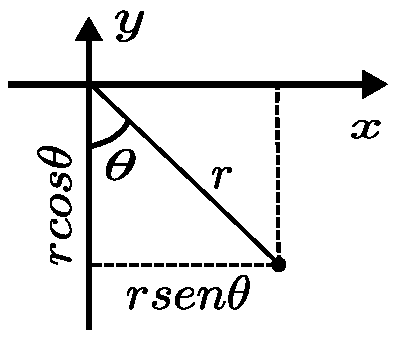
\includegraphics[scale=0.4]{classica-img/pendulo1.pdf}
\end{figure}

Da figura a cima  extrai-se as coordenadas polares. E suas derivadas são:
$$
\begin{array}{ccccccc}
x & = & r \mathrm{sen} \theta & \Rightarrow & \dot{x} & = & \dot{r} \mathrm{sen} \theta + r \dot{\theta} \mathrm{cos} \theta \\
y & = & r \mathrm{cos} \theta & \Rightarrow & \dot{y} & = & \dot{r} \mathrm{cos} \theta - r \dot{\theta} \mathrm{sen} \theta
\end{array}
$$

Da energia cinética e potencial
$$
T = \frac{1}{2}m (\dot{x}^{2} + \dot{y}^{2}) = \frac{1}{2}m ( \dot{r}^{2} + r^{2} \dot{\theta}^{2} ), \ \ \
V = m(-g)y = - mgr \mathrm{cos}\theta
$$
%
Temos que a lagrangeana em coordenadas polares planas
%
$$
L = T - V = \frac{1}{2} m ( \dot{r}^{2} + r^{2} \dot{\theta}^{2} ) + mgr \mathrm{cos}\theta
$$
%
Das equações de movimento
%
$$
\frac{d}{dt} \left( \frac{\partial L }{ \partial \dot{r} }  \right) - \frac{ \partial L }{\partial r} = 0, \quad \quad
\frac{d}{dt} \left( \frac{\partial L }{ \partial \dot{\theta} }  \right) - \frac{ \partial L }{\partial \theta} = 0
$$
Fazendo as derivadas:
$$
\frac{d}{dt} \left( \frac{\partial L }{ \partial \dot{r} }  \right) = \frac{d}{d t} (m \dot{r}) = m \ddot{r}; \quad \quad
\frac{\partial L}{\partial r} = mr \dot{\theta}^{2} + mg \mathrm{cos}\theta
$$
Temos a equação de movimento em relação a $r$:
$$
m \ddot{r} - mr \dot{\theta}^{2} - mg\mathrm{cos} \theta = 0 \Rightarrow \boxed{\ddot{r} - r \dot{\theta}^{2} - g \mathrm{cos}\theta  = 0}
$$
E como:
$$
\frac{d}{dt} \left( \frac{\partial L}{\partial \dot{\theta} } \right) = \frac{d}{dt} (mr^{2} \dot{\theta})  = mr^{2} \ddot{\theta} + 2mr \dot{r} \dot{\theta}; \quad \quad \frac{\partial L}{\partial \theta} = - mgr \operatorname{sen}\theta
$$
Temos a equação de movimento em relação a $\theta$:
$$
mr^{2} \ddot{\theta} + 2mr \dot{r} \dot{\theta} + mgr \operatorname{sen} \theta = 0 \Rightarrow \quad  \boxed{ r^{2} \ddot{\theta} + 2r\dot{r} \dot{\theta} + gr \operatorname{sen} \theta = 0}
$$




b) Suponha que o pêndulo seja lançado de $\theta(0) = \theta_{0}$ com $\dot{\theta}_{0} = 0$. Calcule o valor máximo que a tensão na haste atinge durante o movimento.

\resposta Então, o pêndulo é solto em um ângulo inicial $\theta_{0}$ com velocidade angular $\dot{\theta}_{0} = 0$. Quando passa pelo ponto de equilíbrio a tensão na haste é máxima:
$$
T = F_{p} + F_{c} \Rightarrow mg + m\ddot{\theta} = mg + m \left( - \frac{g}{l} sen \theta_{0}  \right) = mg \left( 1 - \frac{1}{l} sen \theta_{0} \right)
$$



c) Encontre $\theta(t)$ na aproximação de pequenas oscilações supondo $\theta(0) = \theta_{0}$ e $\dot{\theta}_{0} = 0$.

\resposta Utilizando os vínculos ( $r = l$, $\dot{r} = 0$ ) nas equações de movimento, vemos que uma delas se torna familiar no caso de pequenas oscilações:
$$
r^{2} \ddot{\theta} + 2r\dot{r} \dot{\theta} + gr \operatorname{sen} \theta = 0 \Rightarrow \quad l^{2} \ddot{\theta} + gl \operatorname{sen} \theta = 0 \Rightarrow \quad \ddot{\theta} + \frac{g}{l} \operatorname{sen} \theta = 0
$$
Para $\theta << 1$ vale a aproximação:
$$
\mathrm{sen}(\theta) = \sum_{n=0}^{\infty} \frac{\theta^{2n + 1}}{(2n+1)!} = \theta + \frac{\theta^{3}}{3!} + \frac{\theta^{5}}{5!} + (...) \approx \theta
$$
Logo:
$$
\ddot{\theta} + \frac{g}{l}\mathrm{sen} \theta  = 0 \Rightarrow \ddot{\theta} + \frac{g}{l} \theta =  \ddot{\theta} + \omega^{2} \theta = 0
$$
Que é a equação do oscilador harmônico, cuja freqüência é dada por: $\omega = \sqrt{\frac{g}{l}} $. E solução geral é dada por
$$
\theta (t) = A \mathrm{cos} (\omega t + \varphi)
$$
Com $A$ e $\varphi$ constantes fixadas pelas condições iniciais. Para demonstrar que esta é a solução, basta testarmos:
$$
\begin{array}{ccc}
  \ddot{\theta} + \omega^{2} \theta & = & \frac{d^{2}}{dt^{2}} A \mathrm{cos}(\omega t + \varphi) + \omega^{2} A \mathrm{cos}(\omega t + \varphi)   \\
   & = & - \omega \frac{d}{dt} A \mathrm{sen} (\omega t + \phi) + \omega^{2} A \mathrm{cos}(\omega t + \varphi) \\
   & = & - A \omega^{2} \mathrm{cos} (\omega t + \varphi) + \omega^{2} A \mathrm{cos} (\omega t + \varphi) = 0
\end{array}
$$
Portanto a função dada é solução da equação acima. Quanto às constantes, fixemo-las a partir das condições iniciais e tomando $0 \leq \varphi < 2\pi $
%
$$
\begin{array}{ccc}
\theta(0) & = & A \mathrm{cos} \varphi  =  \theta_{0} \Rightarrow A = \frac{\theta_{0}}{\mathrm{cos} \varphi}; \\
\dot{\theta}(0) & = & - \omega A \mathrm{sen} \varphi = - \frac{\omega \theta_{0}}{\mathrm{cos}\varphi } \mathrm{sen} \varphi \\
& = & - \theta_{0} \omega \mathrm{tan} \varphi = 0 \  \  \Rightarrow \  \  \varphi = 0 \mbox{ e } A = \theta_{0}
\end{array}
$$

\textit{Sic}:
$$
\theta(0) = \theta_{0} \mathrm{cos}\omega t
$$


d) Esboce um gráfico mostrando como o período do movimento da partícula varia com a sua energia.


\resposta  $\omega = \sqrt{\frac{g}{l}}$ e a energia total dos sistema é dada por - se expressar esta em termos das variáveis específicadas nas condições iniciais:
$$
E = mgl (1 -  \mathrm{cos} \theta_{0} ) \ \ \Rightarrow \ \ l = \frac{E}{mg(1 -  \mathrm{cos} \theta_{0})}
$$
Logo, como $\omega = \frac{2 \pi}{T}$, temos como expressar o período como função da energia $E$:
$$
T = 2\pi \sqrt{ \frac{E}{mg^{2}(1 -  \mathrm{cos} \theta_{0})} }  \ \approx \ \sqrt{\frac{2 E}{g^{2} m \theta_{0}}}
$$
Que nos fornece o gráfico a baixo.
\begin{figure}[H]
\centering
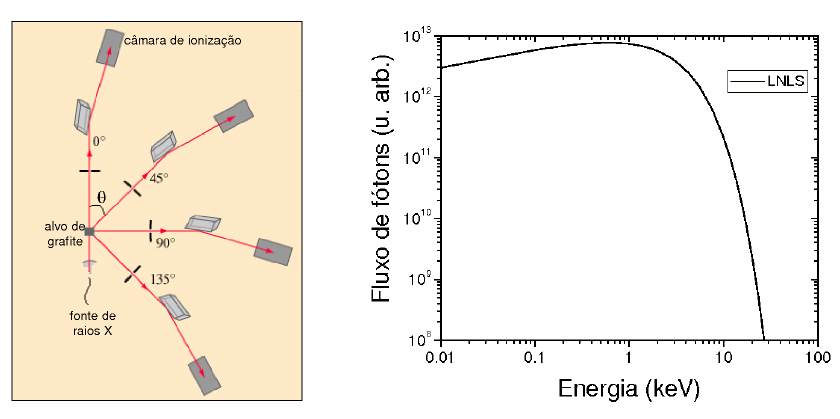
\includegraphics[scale=0.7]{classica-img/energia.png}
\caption{Período em função da energia para o pêndulo na aproximação de pequenas oscilações em torno de $\theta = 0$.}
\end{figure}


\item Um disco uniforme, de seção reta circular de raio $R$, massa $M$ e momento de inércia $I$ (com relação ao eixo perpendicular ao plano do disco e que passa pelo seu centro), encontra-se preso a uma mola de constante $k$, massa desprezível e um certo comprimento de repouso, como é mostrado na figura abaixo. O disco rola sobre a superfície sem deslizar e seu movimento está confinado ao plano da figura.
\begin{figure}[H]
\centering
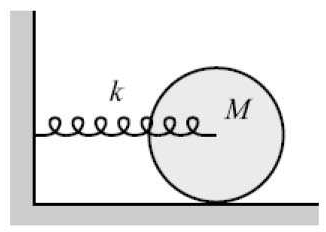
\includegraphics[scale=0.7]{classica-img/mola.png}
\end{figure}

a) Escreva a equação para a energia mecânica do sistema em função da velocidade do centro de massa e da distensão da mola.

\resposta Note que há um vínculo: $\theta = \frac{x}{R} \ \Rightarrow \ \dot{\theta} = \frac{\dot{x}}{R}$.
$$
T = \frac{I \dot{\theta}^{2}}{2} + \frac{M \dot{x}^{2}}{2}; \ \ V = \frac{k x^{2}}{2}
$$
Como a densidade é uniforme: $\sigma = \frac{M}{\pi R^{2}}$.

Apenas para fazer uma observação adicional, calcularei o momento de inércia do cilindro, cujo raio é $R$ e cuja distribuição de massa é uniforme. A distância do eixo do cilindro a um ponto arbitrário será batizada de $r$. O eixo de rotação desse cilindro se encontra no centro deste, de forma que temos a seguinte integral:
$$
\begin{array}{ccl}
  I = \int \int r^{2} dm  & = & \int \int r^{2} \sigma(r) d^{2} r = \int_{0}^{R} \int_{0}^{2\pi} r^{2} d m \\
   & = & \int_{0}^{R} \int_{0}^{2\pi} \frac{M r^{3}}{\pi R^{2}} dr d\theta = \frac{2M}{R^{2}} \int_{0}^{R} r^{3} dr = \frac{2 M R^{4}}{4R^{2}} = \frac{MR^{2}}{2}
\end{array}
$$
Vê-se que:
$$
 E = T + V = \frac{kx^{2}}{2} + \frac{I \dot{\theta}^{2}}{2} + \frac{M \dot{x}^{2}}{2}
 $$
Apenas vou utilizar o vínculo para expressar tudo em termos da coordenada $x$:
$$
 E = \frac{kx^{2}}{2} + \frac{\dot{x}^{2}}{2} \left( M + \frac{I}{R^{2}}  \right) = \frac{kx^{2}}{2} + \frac{3M \dot{x}^{2}}{4}
$$



b) Obtenha a equação de movimento para o centro de massa do disco.

\resposta

Sabemos que:
$$
 L = T - V =  \frac{\dot{x}^{2}}{2} \left( M + \frac{I}{R^{2}}  \right) - \frac{kx^{2}}{2} = \frac{3M \dot{x}^{2}}{4} - \frac{kx^{2}}{2}
$$
A equação de Euler-Lagrange é dada por:
$$
\frac{d}{dt} \left( \frac{\partial L}{\partial \dot{x}}  \right) - \frac{\partial L}{\partial x} = 0
$$
$$
\frac{\partial L}{\partial x} = -kx
$$
$$
\frac{\partial L}{\partial \dot{x}} = \left( M + \frac{I}{R^{2}}  \right) \dot{x} = \frac{3M}{2} \dot{x} \ \Rightarrow \ \frac{d}{dt} \frac{\partial L}{\partial \dot{x}} = \left( M + \frac{I}{R^{2}}  \right) \ddot{x} = \frac{3M}{2} \ddot{x}
$$
Logo, a equação de movimento do centro de massa é:
$$
\left( M + \frac{I}{R^{2}}  \right) \ddot{x} + kx = 0 \ \Rightarrow \ \ddot{x} + \left(\frac{k}{M + I/R^{2}}  \right) x = 0 \ \Rightarrow \ \ddot{x} + \frac{2k}{3M} x = 0
$$


c) Determine a frequência angular de oscilação do centro de massa do disco.


\resposta Através da equação de movimento, vemos que a frequência angular é:
$$
\omega = \sqrt{\frac{k}{M + I/R^{2}}} = \sqrt{\frac{2k}{3M}}
$$


\item Uma partícula de massa $m$ move-se em um potencial $V(r) = -C/(3r^{3})$, sendo $C$ uma constante positiva. Considere que a partícula possua momento angular $L$ diferente de zero.

a) Escreva a equação para a energia mecânica da partícula em termos da distância $r$ à origem, da sua derivada temporal $\dot{r}$, do momento angular $L$, da massa $m$ e da constante $C$.

\resposta A energia cinética de um potencial tipo central é:
$$
T = \frac{m \dot{r}^{2}}{2} + \frac{m r^{2} \dot{\theta}^{2}}{2} = \frac{m \dot{r}^{2}}{2} + \frac{L^{2}}{2 m r^{2}}
$$
Sendo $L = mr^{2} \dot{\theta}$. Para um potencial central vale a expressão:
$$
E = T + V = \frac{m \dot{r}^{2}}{2} + \frac{m r^{2} \dot{\theta}^{2}}{2} - \frac{C}{3r^{3}} = \frac{m \dot{r}^{2}}{2} + \frac{L^{2}}{2 m r^{2}} - \frac{C}{3r^{3}}
$$


b) Considerando os termos que só dependem de $r$ na energia mecânica como um potencial efetivo $V_{ef}(r)$, esboce o gráfico de $V_{ef}(r)$.

\resposta Utilizando a sugestão do enunciado:
$$
V_{ef}(r) = \frac{L^{2}}{2mr^{2}} - \frac{C}{3r^{3}}
$$
O gráfica é
\begin{figure}[H]
  \centering
  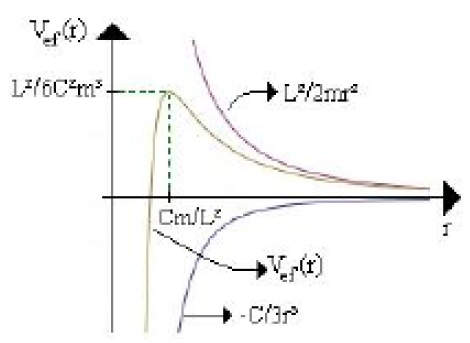
\includegraphics[scale=0.7]{classica-img/potencial}
  \caption{Gráfico do potencial efetivo, $V_{ef}(r)$, juntamente com os gráficos de $\frac{L^{2}}{2mr^{2}}$ e $\frac{-C}{3r^{3}}$.}
\end{figure}

c) Existem órbitas circulares para essa partícula? Em caso afirmativo, determine o raio de cada uma dessas possíveis órbitas e discuta a estabilidade das mesmas.

\resposta De fato, existem órbitas circulares para a partícula, pois:
$$
\left. \frac{\partial V_{ef}(r)}{\partial r} \right|_{r_{0}} = 0 \ \Rightarrow \ \left. \frac{\partial}{\partial r} \left( \frac{L^{2}}{2mr^{2}} - \frac{C}{3r^{3}} \right) \right|_{r_{0}} = \left. \left( \frac{C}{r^{4}} - \frac{L^{2}}{mr^{3}} \right) \right|_{r_{0}}
$$
$$
\Rightarrow \ \frac{C}{r_{0}^{4}} = \frac{L^{2}}{mr_{0}^{3}} \ \Rightarrow \ \left\{ \begin{array}{ccc}
                                           r_{0} & = & 0 \\
                                           r_{0} & = & \frac{Cm}{L^{2}}
                                         \end{array} \right.
$$
A primeira solução não é válida (as funções não são definidas em zero). Portanto, é possível a ocorrência de órbita para:
$$
r_{0} = \frac{Cm}{L^{2}}
$$
Sobre a estabilidade da órbita, devemos analisar a derivada segunda:
$$
\left. \frac{\partial^{2} V_{ef}(r)}{\partial r^{2}} \right|_{r_{0}} = \left. \left( \frac{3L^{2}}{mr^{4}} - \frac{4C}{r^{5}} \right) \right|_{r_{0}} = \frac{3L^{10}}{C^{4} m^{5}} - \frac{4L^{10}}{C^{4}m^{5}} = - \frac{L^{10}}{C^{4}m^{5}} < 0 \therefore \mbox{ a órbita é instável}
$$
Essa informação poderia ser retirada do gráfico, se notarmos que pequenas perturbações do sistema não levam-no de volta ao ponto de equilíbrio.


d) Calcule a energia mecânica mínima, $E_{min}$, acima da qual a partícula vinda do infinito é capturada pelo potencial, ou seja, não retorna mais para o infinito.

\resposta Se $E > V_{ef}(r_{0})$ ocorre a 'captura' da partícula:
$$
V_{ef} = \frac{L^{2}}{2mr_{0}^{2}} - \frac{C}{3r_{0}^{3}} = \frac{L^{6}}{2C^{2}m^{3}} - \frac{L^{6}}{2C^{2}m^{3}} = \frac{L^{6}}{6C^{2}m^{3}}
$$
Essa é a energia mecânica mínima necessária para que uma partícula vinda do infinito seja 'capturada'.









\item Considere um corpo de massa $m$ preso a uma mola de constante elástica $k$ e sujeito a uma força externa $F(t) = F_{0} \mathrm{cos} (\omega t)$. Suponha que o movimento da massa seja unidimensional e despreze as forças de atrito.


a) Escreva a equação de movimento.

\resposta

b) Obtenha a solução geral da equação homogênea, $x_{h}(t)$, e uma solução particular da equação não-homogênea, $x_{nh}(t)$.

\resposta

c) Escreva a solução total $x(t)$ e imponha as condições iniciais $x(0) = x_{0}$ e $\dot{x}(0) = 0$.

\resposta
  
d) Obtenha $x(t)$ no limite $\omega \rightarrow \omega_{0}$, onde $\omega_{0} = \sqrt{k/m}$.

\resposta


\item Considere uma partícula de massa $m$ mmovendo-se sob a ação do potencial central $V(r) = k(r/r_{0})^{4}$ onde $k$ e $r_{0}$ são constantes positivas. Em coordenadas polares o movimento radial é dado pela equação $m\ddot{r} = - d V_{ef}/dr$ onde $V_{ef} = V(r) + L^{2}/(2mr^{2})$ e $L = mr^{2} \dot{\theta}$ é o momento angular perpendicular ao plano do movimento.


a) Faça um esboço do potencial efetivo.

\resposta

b) Encontre a distância $a$ da partícula ao centro de forças para que seu movimento seja uma órbita circular com momento angular $L = 2 r_{0} \sqrt{mk}$. Calcule o valor das energias cinética, potencial e total nesta órbita.

\resposta

c) Calcule o período de rotação deste movimento circular.

\resposta

d) Se a partícula em órbita circular sofrer uma pequena perturbação que não altere o valor de $L$ ela começará a oscilar em torno da órbita original. Calcule o período de pequenas oscilações radiais deste movimento.

\resposta




\end{enumerate}






